



\chapter{Variability in evolution}











\subsection*{Speculative apocrypha}



When a group has dominion over an excess supply of resources, its selective pressures will be lessened by ease of replication without struggle, less offspring persisting and passing on variation.

This causes the ever-present potential for variability to become manifest, resulting in a smooth spectrum of divergences and variations. 

As the population expands to meet the supply of resources, the selective pressures begin to return, and what has become a sprawling range of variants once more becomes subject to the formative influence of selection. This begins to ``lock in'' an array of increasingly distinct sub types as the convergence to local optima commences. 

As species begin to move at odds with one-another, there begins competition for the once shared domain. Competitive exclusion may drive types into various distinct sub-niches. But where there is direct overlap, the Matthew effect takes hold, with those species that have some advantage benefiting secondarily from an increase of dominance. 

In this way, what became a huge multiplicity of forms gets reduced. Only a few will persist beyond the day after tomorrow. Only those with some edge, or that were able to secure the early monopoly.

In this way, a substantial easing of selective pressures can cause a stepwise morphological change consistent with the paradim of punctuated equalibria. Much speculation could be made into the possable causes of such a change of conditions. 

The expansion of a genus into a un-exploighted region
Perhaps like the first insects on dry land with a multitude of mosses and small shrubs to feast on. 
Even the first vertebrates that learned how to eat insects. 

Those left after a mass extinction event
Like the small mammals who inherited great swaths of fertile forests after dinosaurs were wiped out at the KT boundary. 

There is speculation that the Cambrian explosion was triggered by some combination of a huge global ice age and a great surplus of oxegen

Speculation has also been made that the evolutionary scale transition from prokaryotes to eukaryotes took place at a time of great surplus oxygen. 

Going beyond the domain of organic life, emergence and divergence of viral models may have followed a similar trajectory. A great variety of models were trialed during a flurry of funding and research into HIV in the early 90s. Over time, only a hand full of these went on to become commonplace.  




Qualitatively, we see that something like this has happened at various times across differing domains. In the first few million years after the cambrian explosion, there were a great variaty of arthropodic forms. 24 classifications have been counted amongst the remains of the Burgess shale. Over time this number was reduced to four main structures: chelicerata (arachnids), crustacea (crustaceans), hexapoda (insects and springtails), and myriapoda (millipedes and centipedes). For about half of the time since then, there were also trilobites, but these eventually dies out. 



\begin{figure}[h!]
    \centering
    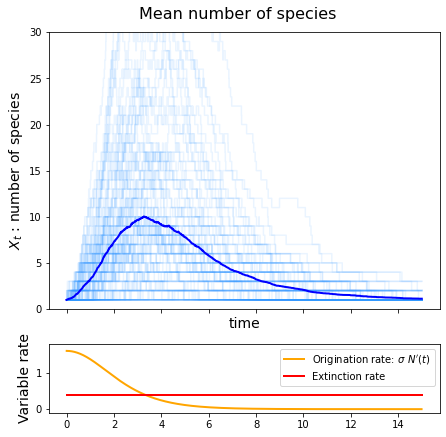
\includegraphics[width=0.7\textwidth]{chapter8/IMG_ch8/LSMean} % Adjust the width as needed
    \caption{Realisations of the logistic speciation model. Many realisations are shown in light blue. Their average is numerically calculated from these and shown in dark blue. It can clearly be seen that this model exhibits a period of heightened diversification when resources are relatively abundant before seeing a reduction as remaining capacity becomes scarce.  In real evolutionary processes, the latter stage of this procedure might be characterised by a smooth range of types diverging into a few distinct and optimised species which then compete and become subject to the Matthew effect.  Then, either a small number of the fixed types win out, or a number each find slightly different ecological niches to occupy.}
    \label{fig:single_figure}
\end{figure}



\section{Push of the past and Pull of the present}


With regards to the standard birth death process in which the condition of survival to the present is imposed (Quoting R.  Mann and G. Budd, who themselves were overviewing the topic introduced by Nee et.  al.):


\begin{quotation}
\noindent
"The POTPa emerges as a feature of diversification by the fact
that all modern clades (tautologically) survived until the present
day. This singles them out from the total population of clades
that could be generated from any particular pair of background
birth and death rates: clades that happened by chance to start off
with higher net rates of diversification have better-than-average
chances of surviving until the present day. As Nee et al. (1994a)
put it, such clades “got off to a flying start”; and they accumu-
late species faster than one would expect. Once clades become
established, they are less vulnerable to random changes in the
observed diversification rate, and this value therefore tends to re-
vert to the background rate through time. Long-lived clades thus
tend to show high observed rates of diversification at their origin,
which then decrease to their long-term average as the present is
approached."
\end{quotation}

\noindent
In their paper, "History is written by the victors," R. Mann and G. Budd propose that the push of the past (POTPa) is an underappreciated phenomenon in the paleontological literature, which delves into mass radiations following mass extinctions.
Without directly opposing their work, I present a model that illustrates a dynamic of variable-rate evolution, which also seeks to shed light on the higher origination rates of species following extinctions and events of ecological instability more generally \cite{bak1991self} \cite{fisher1929genetical}\cite{budd2018history}.







\section{Logistic speciation}







The number of individuals, or size of a population grows logistically according to standard logistic growth:
$$\ddt{N} = rN\lrb{1-\frac{N}{K}}.$$
The size of population, $N(t)$ is taken to be a continuous variable, a real number. It is assumed that this number of individuals is large compared to the count of species within the total group.\par

Types beget further variations in a descent of speciation that behaves as a Yule pure birth process. That is, given a number of types, $\yt$, initially 1, changes occur as defined: 
$$\pr{\yy_{t+\delt} - \yy_t = 1} = \beta \yy_t \delt + o(\delt)$$
taken in the limit, $\delt\to 0$. In the standard Yule process --- originally specified in 1924 to model the development of species --- $\beta$ is a constant value. Here however, we define this rate of speciation as a function of time. 
$$\beta \equiv \beta(t).$$
Such a step has been made before. Both in the field of evolutionary modeling, and elsewhere. If we were to set $\beta = \ee^{-t}$, the mean of $\yt$ would be described by the deterministic Gompertz model, introduced in 1825 \cite{gompertz1825xxiv}.\par

It doesn't appear that anyone has yet published a version of the model that uses the logistic function. There are a few ways of doing this, for now we will assign $\beta(t)$ the form, 
\begin{equation}
\label{rate1}
\beta(t) = \sigma\lrb{K - N(t)}.
\end{equation}
It serves as an index for the relative abundance of resources experienced by the population.\par

When $N(t)$ is small compared to the carrying capacity of the ecosystem, $K$, $\beta(t)$ is towards the higher end of it's range; species beget species with greather fecundity. We will later explore other options for the birth rate, for example, it may be sensible to ascribe the formula as $\beta(t) = \sigma\cdot \dd N/\dd t$ which would see the highest rate of division at the time of most rapid expansion --- perhaps this makes more sense than the fastest speciation beginng when the population is smallest. But for now let us continue with formula (\ref{rate1}). 

\vspace{10pt}
\hrule
\vspace{10pt}
\noindent
\begin{quotation}
\noindent
\textbf{Aside:} While writing this out, I am starting to wonder if the rate of population expansion is actually orders of magnitude faster than that of speciation. What if the logistic growth doesn't itself spur on type divisions, but instead lays out the potential for them. In this case, it would be incorrect to account for high early rates of speciation with the period of logistic expansion, however, such an expansion may mark the initial condition of a more DDD like model (density dependent diversification) such as the one we were initially working on.  \par

Could it be there is some effect whereby a homogeneos population experiences a saftey in numbers effect, i.e. a larger group has greater control of resorrces and its individuals are more protected from predators and competitors. In this case, the propensity to vary could be inflated. Then as the homogeneos group divides into ever smaller and smaller sub groups, they become more vulnerable --- this leading to harsher selection pressures and lower diversification rate.  
\end{quotation}
\vspace{10pt}
\hrule  
\vspace{10pt}

\noindent
The topic of variable variation in a group has been discussed by many thinkers: from Lamarck at the turn of the 19th centuary, to Darwin in the late 19th centuary; a number of more modern contributers such as S. J Gould in the latter 20th centuary. 
Somewhere in the middle, Ronald Fisher in his 1929 book, The Genetical Theorey of Natural Selection, implies that variations to a type are in constant and abundant supply, and that it is the harshness of environmental conditions in conjunction with sexual mixing which constantly work to quell this significant tendancy for genomes to become irretrievably disprate. 




According to Ronald Fisher, variations to the norm of a given type are in constant and abundant supply. It is the harshness of environmenal conditions which prevents many of them from becoming established; selection pressure supports adhearnce to a current optimal form. But when the selection pressures are lesser, when for example there are more comfortable conditions in the form of a fresh abundance of resources available to the population, variations to the norm are more likely to survive. 
\begin{quotation}
It is known by the experience of breeders that species which recieve superabundant nourishment, and in general a surplus of protection and care, immediately tend in the most marked way to develop variation, and are fertile in prodigies and monstrosities." (Nietzsche beyond good and evil section 262).
\end{quotation}

\begin{quotation}
"To maintain a stationary variance, fresh mutations must be available in each generation." (R. Fisher, the genetical theory of natural selection)
\end{quotation}

The whole thing is reminiscent of the concept described by Ilya Prigogine of dissipative structures. The idea being that where a flow of energy of matter is seen, structures can emerge which apparently go against the second law of thermodynamics. Locally, order can emerge as a spontaneous reduction in entropy. And this emergence is characterised by chaotic dynamics, its exact formation arising influenced by small fluctuations whos effects magnify and propergate.\par
Examples of dissipative structures can be seen throughout the natural world. It seems that one is the evolution of life into a multitude of forms and varieties.





\section{Model specification and results (no death case analytic soloutions)}

The following model is a version of the Yule process where the division rate, $\beta$, is a function of time. $\yt$ describes the number of species and it changes in continuous time according to the transition probabilities:


\begin{align}
\label{cases1}
\begin{split}
\pr{\yy_{t+\delt} - \pr{\yt} = 1} = \beta(t)\delt\yt + o(\delt)\\
\pr{\yy_{t+\delt} - \yt = 0} = 1 -  \beta(t)\delt\yt + o(\delt)
\end{split}
\end{align}
defined for $\delt\to 0$. \par
$N(t)$ is an index for the total population size, of individuals, constituting the sum of those in each $\yt$ species. Assuming the overall population is large, even from the beginning, $N(t)$ is defined as a real number. Starting at $N(0) = N_0$, the population develops acording to standard logistic growth: 
$$\ddt{N} = rN\lrb{1 - \frac{N}{K}};$$
Which permits description by the known formula, 
$$N(t) = \frac{K\ee^{rt}}{\xi + \ee^{rt}},$$
with the constant combination, $\xi = K/N_0 - 1$.\par
As discussed above, the model is set up to capture a variable speciation rate, and $\beta(t)$ varies with $N(t)$ to account for selection pressure --- higher when resources are less scarce. The exact form of $\beta(t)$ is a potential subject of experimentation. For now, we will  develop the case where
\begin{equation}
\label{basicRate1}
\beta(t) = \sigma\lrb{K-N(t)},
\end{equation}
but later, the following alternatives may also be explored:
\vspace{10pt}
\hrule
\vspace{10pt}
\noindent
\textbf{Alternative speciation rates}
\begin{itemize}
\item $\beta_2(t) = \sigma\lrb{K-N(t)} + \eta$,\\ ($\eta$ constant)
\item $\beta_3{t} = \sigma \ddt{N}$
\item $\beta_4{t} = \sigma \ddt{N} + \eta$
\item $\beta_5(t) = \sigma\lrb{K_t-N(t)}$,\\ with $K_t$ behaving according to some random switching regime (this may be a little too ambitions)
\end{itemize}
It may make sense for the speciation rate to depend on the rate of population increase rather than simply its size compared to availability of resource. With rapid individual replication, more opportunities are present for specific mutation events.\par
The incorporation of $\eta$ in case $\beta_2$ \& $\beta_4$ represents some baseline rate of variation, approached to at late time at the $N(t)$ reaches its steady state. This seems fitting to represent some underlying disequalibria in an ecosystem.  
\vspace{10pt}
\hrule
\vspace{10pt}

\noindent
With the above formula for $N(t)$, we can also write the division rate, (\ref{basicRate1}), as 
$$\beta(t) = \sigma\lrb{K - \frac{K\ee^{rt}}{\xi + \ee^{rt}}}$$
simplifying to 
$$\beta(t) = \sigma K \frac{\xi}{\xi + \ee^{rt}}$$


\subsection{Expectiation $\mean{\yt}$}
In the chosen case where $\beta(t)$ tends to 0 at late time, the final state of the process, $\yy_{t\to\infty}$, will arive at some fixed value. This could be thought of independently as a random variable with some mean, variance and distribution. Knowing more about this asymptoitc stationary distribution, we can ask questions surrounding how its nature depends on the parameters and their inyterplay. Here we will compute the mean, but we can do better than mearly compute its late time measure. It turns out quite straightforward to foumulate the expected value as a function of time; in this way we can see how the final position is approached. \par

If we consider how the expectation of $\yy_t$ changes over some vanishing interval, $\delt$, the mean after the interval is equivalent to the mean before plus the expected change;
\begin{equation}
\label{ExpectChange1} 
\mean{\yy_{t+\delt}} = \mean{\yt} + \mean{\yy_{t+\delt} - \yy_t}.
\end{equation}
And this latter term, the change, can be analysed in tems of the definition of the dirctete expectation, along with the possible cases and their associated probabilities (see (\ref{cases1})):

$$ \mean{\yy_{t+\delt} - \yy_t} = 0 \cdot \lrbs{1 -  \beta(t)\yt\delt} + 1\cdot \lrbs{\beta(t)\yt\delt} + o(\delt)$$
Ommitting the $\delt$, this simplifies to
$$ \mean{\yy_{t+\delt} - \yy_t} =  {\beta(t)\delt\yt} $$
which is equivalent to 
$$ \mean{\yy_{t+\delt} - \yy_t} =  {\beta(t)\delt\mean{\yt}}$$
(by taking the expected value of each side). Hence, with (\ref{ExpectChange1}), we can write
$$\frac{\mean{\yy_{t+\delt}} -  \mean{\yt}}{\delt} =    {\beta(t)\mean{\yt}},$$
or in the limit $\delt \to 0$,
$$\ddt{} \mean{\yy_t} = \beta(t) \mean{\yt}.$$
This is a seperable equation $\to$
$$\int\frac{1}{\mean{\yt}}\dd \mean{\yt}  = \int \beta(t) \dd t =  \sigma K \xi \int \frac{1}{\xi + \ee^{rt}} \dd t.$$
And with 
\begin{equation}
\label{intBetaT}
\int \frac{1}{\xi + \ee^{rt}} \dd t =\frac{1}{\xi} \lrb{ t - \frac{1}{r} \ln\lrb{\xi + \ee^{rt}} },
\end{equation}
it permits a solution in the following way.
$$\ln\lrb{\mean{\yt}} =  \sigma K\lrb{ t - \frac{1}{r} \ln\lrb{\xi + \ee^{rt}} }  + \text{const},$$
$$\mean{\yt} = C_0 \ee^{\sigma K\lrb{ t - \frac{1}{r} \ln\lrb{\xi + \ee^{rt}} } }.$$
The constant, $C_0$, is fixed with the initial condition, $\mean{\yy_0} = 1$:
$$C_0 = \ee^{\frac{\sigma K}{r} \ln\lrb{ \xi+1}}.$$
So
$$\mean{\yt} = \ee^{\sigma K \lrb{ t - \frac{1}{r} \ln\lrb{\xi + \ee^{rt}} +\frac{1}{r}\ln\lrb{\xi + 1} }}$$
and with some rearrangment, 
$$\mean{\yt} =  \ee^{\sigma K t} \lrb{\frac{\xi + 1}{\xi + \ee^{rt}}}^{\frac{\sigma K}{r}}.$$ 






\subsection{Probability generating function $G_{\yt}(z, t)$}

In validating a model like this with observational data, there are a number of measures that could be considered. The mean number of species through time could be of use, but we will no doubt be better equiped with knowledge of the full distribution of $\yt$. For this, and other metrics such as the variance, we can employ the probability generating function (PGF).
$$G_{\yt}(z,t) = \sum^{\infty}_{i=0} \pr{\yt = i} z^i $$
Along with being a means of verifying our mean formula,
$$\mean{\yt} = \dda{G}{z}\bigg|_{z=1} = \sum_{i=1}^{\infty} i \pr{\yt = 1} (1)^{i-1},$$
the probability of $\yt$ being in any state, $i$, can be computed with repeated differentiation:
\begin{equation}
\label{diston}
\pr{\yt = n} = \frac{1}{n!}\frac{\partial^n G}{\partial z^n}\bigg|_{z= 0}
\end{equation}
For the present system, the iterative diferentiation happens to generalise as a formula. Details of this can be seen below. For now, let us focus on deriving the PGF.

\subsubsection*{Forward Kolmogorov equation}

The forward Kolmogorov equation for this system is essentially the same as that of the pure birth process. All which differes is that here the rate is a function of time. It is derrived in the following way by considering what occurs in a vanishing interval of duration $\delt$. Denoting $p_i(t) = \pr{\yt = i}$,
$$p_i(t+\delt) = \beta(t)(i-1) \delt p_{i-1}(t) + \lrb{1 - \beta(t) i \delt} p_i(t).$$
Rearranging, and taken in the limit, $\delt\to 0$, this becomes
$$\ddt{p_i(t)} = \beta(t)(i-1) p_{i-1} - \beta i p_i.$$
By a procedure covered in section (TO ADD), the FKE can be transformed into an equation describing the probability generating function: 
$$\frac{\partial G}{\partial t} = \beta(t) z(z - 1) \frac{\partial G}{\partial z}$$  
Which, despite the form of $\beta(t)$, does permit a solution via the method of characteristics. Details of the process are covered elsewhere, but it boils down to: making a change of variables, then solving the characteristic equations for a chosen set of initial conditions. \par
Here, the change of variables is 
$$G(z,t) \equiv G\lrb{s((z,t), \tau(z,t))} = G(s,\tau);$$
initial conditions can be set to
\begin{align}
\label{charICs}
z(s, \tau = 0) = s, && t(s, \tau = 0) = 0;
\end{align}
and the characteristic equations are
\begin{align}
\dda{G}{\tau} &= 0,\\
\dda{t}{\tau} &= -1,\label{char12}\\
\dda{z}{\tau} &= \beta(t)z(z - 1).\label{char13}
\end{align}
The first two tell us that $G(s,\tau)$ is purely a function of $s$,
$$G(s,\tau) = \phi(s);$$
and (\ref{char12}) that $t = -\tau$. If we assume there to be just a single initial species, $\yy_0 = 1$, then for time $t=0$, the probability generating function will take the form,
$$G(z, 0) = z.$$
And with this, along with the initialcondition, $z(s, \tau = 0) = s$, we can fix $G$ in terms of $s(z,t)$ as 
$$G(s, \tau) = s.$$
This will prove essential in obtaining the final formula. To now find the expression of $s(z,t)$ in terms of our functional variables, $z$ \& $t$, we turn to the last characteristic equation, (\ref{char13}). With $t = -\tau$, it seperates as,
\begin{equation}
\label{char3int}
\int\frac{1}{z(z-1)}\dd z = \int \beta(-\tau) \dd\tau.
\end{equation}
As the integral of $\beta$ with respect to $t$ is known --- (\ref{intBetaT}) --- with $\dd \tau = -\dd t$, the RHS above can be delt with as,
$$\int \beta(-\tau)\dd \tau = - \int \beta(t) \dd t.$$
Thus, (\ref{char3int}) is evaluates to
$$\ln\lrb{\frac{z-1}{z}} =   \sigma K \lrb{\tau + \frac{1}{r}\ln\lrb{\xi + \ee^{-r\tau}}  } + \text{const}.$$
The constant can be fixed with initial conditions, (\ref{charICs}),
$$\text{const} = \ln\lrb{\frac{s-1}{s}} - \frac{\sigma K }{r} \ln\lrb{\xi + 1},$$ 
so,
$$\ln\lrb{\frac{z-1}{z}} =   \sigma K \lrb{\tau + \frac{1}{r}\ln\lrb{\xi + \ee^{-r\tau}}  } +  \ln\lrb{\frac{s-1}{s}\lrb{\xi + 1}^{-\frac{\sigma K }{r} } }.$$
Rearranging for $s$:
$$s = \lrb{1 - \lrb{\frac{z-1}{z}} \ee^{-\sigma K \tau} \lrb{\frac{\xi + 1}{\xi + \ee^{-r\tau}}}^{\frac{\sigma K}{r}} }^{-1}.$$
Hence, 
\begin{equation}
\label{PGF1} 
G(z, t) = \frac{z}{z + (1 - z) \ee^{\sigma K t} \lrb{\frac{\xi + 1}{\xi + \ee^{rt}}}^{\frac{\sigma K}{r}}}.
\end{equation}

\subsubsection*{Connecting to the mean foumula}
For simplicity, we can represent (\ref{PGF1}) by 
$$G(z, t) = \frac{z}{z\lrb{1 - \Psi(t)} + \Psi(t)},$$
with
$$\Psi(t) =  \ee^{\sigma K t} \lrb{\frac{\xi + 1}{\xi + \ee^{rt}}}^{\frac{\sigma K}{r}}.$$
To use the PGF, $G(z,t)$, for computing the mean, $\mean{\yt}$, one simply needs to differentiate partially with respect to $z$, then substitute $z=1$. Since $\Phi(t)$ does not depend at all on $z$, it can be treated as constant during the differentiation. A straightforward application of the quotient rule yields
$$\partial_z G = \frac{z\lrb{1 - \Psi}  + \Psi  - z(1 - \Psi) }{\lrb{z\lrb{1 - \Psi} + \Psi}^2} = \frac{\Psi}{\lrb{z\lrb{1 - \Psi} + \Psi}^2}.$$
Then, with $z = 1$,
$$\partial_z G |_{z=1} = \Psi$$
And in fact, we recognise that $\Psi(t) \equiv \mean{\yt}$. 



\subsection{Full distribution of $\yt$}

To compute a probability that the process, $\yt$, is in state $n$, we can use formula (\ref{diston}). It requires differentiating the probability generating function $n$ times... Just above, we got off to a flying start by finding the first of these iterations:
$$\partial_z G = \Psi \lrb{z(1-\Psi) + \Psi}^{-2}.$$
From here on, a pattern emerges.
\begin{align*}
\partial_z G &= \Psi \lrb{z(1-\Psi) + \Psi}^{-2}\\
\partial_{2z} G &= 2\Psi (\Psi -1 ) \lrb{z(1-\Psi) + \Psi}^{-3}\\
\partial_{3z} G &= 2\cdot 3\Psi (\Psi -1 )^{2} \lrb{z(1-\Psi) + \Psi}^{-4}\\
&\hspace{45pt}\vdots\\
\partial_{nz} G &= n!\Psi (\Psi -1 )^{n-1} \lrb{z(1-\Psi) + \Psi}^{-(n+1)}
\end{align*}
To obtain the full distribution of states, we must only substitute $\partial_{nz}$ into formula (\ref{diston}), evaluating the result at $z=0$:
$$\pr{\yt = i} = \Psi^{-n}\lrb{\Psi- 1}^{n-1}$$ 
And with substitution of $\Psi = \Psi(t)$,
$$\pr{\yt = i} = \lrb{ \ee^{\sigma K t} \lrb{\frac{\xi + 1}{\xi + \ee^{rt}}}^{\frac{\sigma K}{r}}}^{-n}\lrb{ \ee^{\sigma K t} \lrb{\frac{\xi + 1}{\xi + \ee^{rt}}}^{\frac{\sigma K}{r}}- 1}^{n-1}$$ 
























\section{Pimental}











\subsection*{Observed experimental dynamics}

Pimentel et al. devised and ran an experiment in which two populations of flies are pitted against each other in a fight for domination and ultimately, survival. \cite{pimentel1965selection}
\cite{hutchingson2018ecological} Suppose you placed a colony of houseflies (Musca Domestica) in one side of a boxed enclosure; a competing number of Blowflies (Phaenicia) at the other. What would eventually happen given an ample but finite supply of food to the container? Before long you would see a niche domination by one of the species. The arrangement being unstable, either the house or blow fly population would eventually see-off the other.\par
Pimentel and his colleagues did something clever to augment the dynamics of this experiment: they contrived an enclosure, take the original box, but with a myriad of internal sub-compartments. A kind of three-dimensional maze of tunnels and mini chambers. Such arrangement permits a desirable property to the enclosure -- with the populations initially placed at opposing sides, eventual communication by contact, interaction is delayed by a period greater than the average lifespan of either species. That is, in the months taken for the dissipation of a species from one side to the other, multiple generations ensue. But why is this desirable?\par
By slowing the potential spread of the species, Pimentel introduces the constraint that given a total domination is arrived at, it can not be won in a time of only one or a few fly lifespans. The war must be won over succeeding generations; grandchildren's grandchildren, all fighting for the same cause. And this allows for the hand of Darwinian selection to come into play.\par
An observation of this contrivance saw the following dynamic. Blowflies were pushed almost to extinction by the initially superior abounding of Musca Domestica, but then, the tides turned... From the brink, the blowfly under-dogs managed to claw back their footing and eventually overthrow the advances of their adversaries.\par
It is hypothesised that during this squeeze of reduced population, the blowflies began to positively select, amongst their limited numbers, for the abilities favouring direct competition with their adversaries. The houseflies, doing well as they were, were subject to no such winds of channelling selection; they became complacent whilst their foes grew strong; cut into shape by a harshly oppressive environment.\par
It has not yet been achieved experimentally, but Pimentel has posed that perhaps given the rightly arranged enclosure, an oscillation could be set up. One in which the upper hand continually passes from the dominion of one side to the other. Each being pushed to the brink, moulded to competitive advantage in times of scarcity -- a continual arms race for survival.\\

\noindent
Can we set up a mathematical model that exhibits such an interplay?\\

\subsection*{Mathematical model}
\noindent
Consider two populations competing for space in the finite domain they both occupy. Define the count of one of the populations (label it ``$a$'') as $(A_t)_{t\in\mathbb{N}\cup \{0\}}$; likewise representing the opposing population, $b$, by a count, $B_t$. Finiteness of the enclosure is imposed by the condition that $A_t + B_t \leq N$, for some maximum capacity, $N$. Population sizes, $A_t$ and $B_t$ will be defined as discrete time Markov processes. For now we will focus our attention on $A_t$, and set up the initial condition as $A_0 = B_0 = N/2$ ($N$ even), leading to the simplifying relation, $B_t = N - A_t$. $A_t$ will have the following transition probabilities:

$$
p_{ij} = \text{Prob}\{A_{t+1} = j | A_{t} = i\} =
\begin{cases}
q_a = \frac{i}{N}(1-p_b), & \text{ for } i = j+1\\
q_b = \left( 1 - \frac{i}{N}\right) (1-p_a), & \text{ for } i = j - 1\\
q_c = \frac{i}{N}p_b + \left( 1 - \frac{i}{N}\right) p_a, & \text{ for } i = j\\
0, \text{ otherwise}\\
\text{if } 0 < i < N; \text{ then for } i =0 \text{ or }i = N:\\
1, & \text{ for } i = j\\
0, \text{ otherwise.}\\
\end{cases}
$$
$p_a$ and $p_b$ to be introduced momentarily, these emerge with the following step rules, viewed from the perspective of $A_t$: 
\begin{quotation}
\noindent
With probability $i/N$, make the decision to move forward provided conditions afford it; wp $1-i/N$, likewise, the opponent will make such a choice, potentially forcing you back one.\\

\noindent
If you have decided to attempt an advance -- do so, unless you are blocked (This happens with probability, $p_b$). \\

\noindent
Given the opponent is advancing, you block them with probability, $p_a$. If unsuccessful, you are forced back a step. \\

\noindent
If a block is effective, both parties remain steady; $A_{t+1} = A_t$.
\end{quotation}
Then, suppose that this capacity to resist, encoded in the probabilities $p_k$ for $k = a,b$, are dependant on the variables, $R_k$:
\begin{align*}
p_a(R_a, R_b) = \text{max}\left\{ 0, 1 - \frac{R_b}{R_a}\right\}\\
p_b(R_a, R_b) = \text{max}\left\{ 0, 1 - \frac{R_a}{R_b}\right\}
\end{align*}
Values, $R_k$, represent the capacity of members in population ``k'' for intraspecific competition with the opposing group. For example, if $R_a \gg R_b$, population $a$'s efficacy in blocking an advance of $b$ individuals will be high ($0\ll p_a < 1$); in this case we will simultaneously have that $p_b = 0$. \par
Resistance capacities, $R_k$, are driven to increase when the associated population is in a minority. The values get updated at each time step by the following rule.
$$R_{k, t+1} =R_{k, t} + \mu\Delta R_{k, t},$$
according to some evolution rate, $\mu$.\par
$\Delta R_{a, t}$, and $\Delta R_{b, t}$ are defined as follows.
\begin{subequations}
\begin{equation}
\Delta R_{a, t} = \text{max}\left\{ 0, \left(\frac{B_t}{A_t}\right)^\alpha\right\} = \text{max}\left\{ 0, \left(\frac{N - A_t}{A_t}\right)^\alpha\right\},
\label{Ra}
\end{equation}
\begin{equation}
\Delta R_{b, t} = \text{max}\left\{ 0, \left(\frac{A_t}{B_t}\right)^\alpha\right\}= \text{max}\left\{ 0, \left(\frac{A_t}{N - A_t}\right)^\alpha\right\},
\label{Rb}
\end{equation}
\end{subequations}
Notice that $\Delta R_{k, t}$ is non-zero and positive, but only when population $k$ is in the minority (less than $N/2$), otherwise it is 0. ``Resistance'' or intraspecific competitive advantage is increased when the population is squeezed into a corner. In this state, most of the competitive interactions experienced by members of the smaller population will be with members of their opposition. The theory goes that this will induce a drive for positive natural selection towards more favourable odds in such a situation. On the other side of the enclosure, however, the majority population enjoy a state in which more of their competitive interactions are interspecific -- with their own kind.\par
As you can see in (\ref{Ra}) and (\ref{Rb}), the rate at which this evolutionary drive occurs increases the closer a population draws towards extinction. Logically, one might expect this rate of increase to be quite simply proportional to the fraction of intraspecific against interspecific meetings, but as an addition, it proves inciteful to augment this basic rate by an exponent, $\alpha$.-- High values of $\alpha$ corresponding to extreme growth in resistance close to the absorbing states, 0, and $N$. We will think of $\alpha = 1$ to be the physical case; $\alpha > 1$ will be considered in pondering the nature and consequences of criticality.\par
\begin{figure}[H]
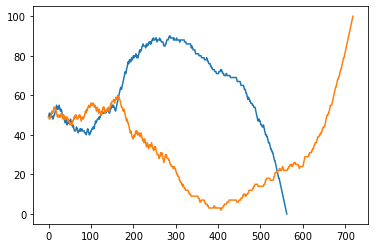
\includegraphics{chapter8/IMG_ch8/pow1N100mu10}
\caption{$\alpha = 1$, $N = 100$, $\mu = 10$. Two realisations of the process. The reversal can clearly been seen in each case.}
\label{2runs}
\end{figure} 

\subsection*{Results}
Running simulations of the model, for now with $\alpha = 1$, we see that the dynamics can indeed resemble what was observed by Pimentel. Both of the two realisations in figure \ref{2runs} display the same kind of behaviour: after some light initial back and forth, one of the populations grows to a position of significant advantage. But it doesn't last. Trained for intraspecific competition, the oppressed population makes a striking comeback, completely overthrowing their adversaries.\par
This was also observed in the experiment; Blowflies come out on top despite initially being pushed to the brink.\\






\noindent
During the last couple of cycles, before fixation, population counts edge ever so close to the boundary. Here, like with the initially critical poise of Fig. \ref{nodisp2runs}, there is a balance between directive forces; resistance of the comparatively supressed population grows to such an extent that the heavy advantage of their adversaries, is muted. And in this arrived at state of poised criticality, like in the previous case, we see a divergence. The two trajectories, as expected, begin to be swayed by subtle underlying disturbances of stochastic undulations.


\begin{figure}[]
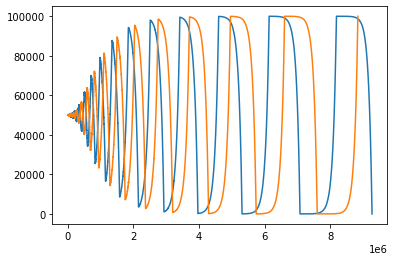
\includegraphics{chapter8/IMG_ch8/pow10N10e5mu1 2 runs 20e3 no displacement}
\caption{$\alpha = 10$, $N = 10\mathrm{e}5$, $\mu = 1$.  Notice that when the two populations start out well-matched, two parallel realizations of the model diverge more substantially than when the initial state involves a bias. Here we see exactly that. The orange and blue lines represent two different stochastic simulations of the model. Because they begin near the critical region of the model, the future trajectory is much more influenced by the cumulative effect of those initial stochastic influences than might otherwise be the case. In the plot below, you can see a red line depicting the critical zone of the model over time. Being near this line is analogous, in deterministic modeling, to having a high Lyapunov exponent.}
\label{nodisp2runs}
\end{figure} 


\begin{figure}[]
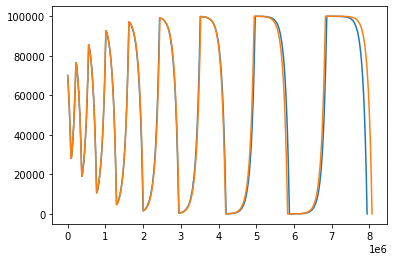
\includegraphics{chapter8/IMG_ch8/pow10N10e5mu1 2 runs 20e3 displacement}
\caption{$\alpha = 10$, $N = 10\mathrm{e}5$, $\mu = 1$.  As mentioned in the caption of the figure above, when trajectories are started with a bias (one species in the majority), repeated simulations will generally stay closer for longer, only diverging near times of extinction. The critical region plays a role in amplifying small differences in stochastic unfolding.}
\label{disp2runs}
\end{figure} 

To get a more clear understanding of what's really going on here we can actually quantify and map this position of criticality over the course of an experiment. By definition, the system is poised at such criticallity exactly when the likelyhood of making a step up vs down is identical:

\begin{equation*}
q_a = \frac{i_c}{N}(1 - p_b) = \left(1 - \frac{i_c}{N}\right) (1 - p_a) = q_b
\end{equation*}
$i_c$ representing the system state at which there is criticality. From this, taking the fact into consideration that $p_a$ and $p_b$ are non-zero with mutual exclusivity, we can derive the relation: 

$$
i_c = 
\begin{cases}
N\dfrac{1 - p_a}{2 - p_a}, &\text{ when } p_a > 0 \text{ and } p_b = 0  \\
N\dfrac{1}{2 - p_b}, &\text{ when } p_b > 0 \text{ and } p_a = 0 \\
\end{cases}
$$

Bearing in mind that $p_a$ and $p_b$ depend on $R_a$ \& $R_b$, and that these are computed as realisations in a stochastic process, the above formulae are not as analytic as they seem. That being said, it is quite straightforward to generate step by step values of the critical state $i_{c, t}$ computationally. These are visible in red over the standard trajectory of the model in figure \ref{redone}. 




\begin{figure}[H]
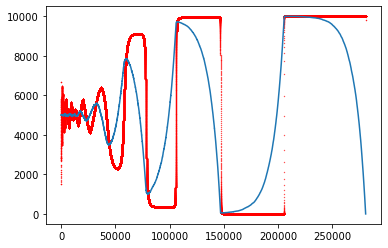
\includegraphics{chapter8/IMG_ch8/pow3N10e4mu1 critical}
\caption{$\alpha = 3$, $N = 10\mathrm{e}4$, $\mu = 1$. The changing critical saddle is depicted in red. When trajectories are close to this line, small perturbations take on a greater significance.}
\label{redone}
\end{figure} 

If we make a qualitative comparrison beteen whats going on in figure \ref{redone}, and in figures \ref{nodisp2runs} \& \ref{disp2runs}, we can see quite clearly, that in \ref{nodisp2runs} \& \ref{disp2runs} trajectories have a propensity to diverge from one another ecaxtly when the state $A_t$ is near criticality.\par
This toughes the essence of what these notes have been trying to get at: near criticality, the future of a system becomes sensitive, succeptible, light underlying stochastic influences. 


\subsection*{Cellular automaton visualisation}

After formulating the model analytically (note: a model has previously been proposed,  \cite{pease1984evolutionary} but the above model wasn't inspired by this and differs in form),  I thought it would be a good idea to produce a spatial version in the form of a sellular automaton. You can see the results of this is the figure here. Blue and red squares represent houseflies and blowflies respectively. This was coded in C++ using the SFML (Simple fast media layer) library which does low-level graphics. 



\begin{figure}[H]
    \centering
    % First row of four images
    \begin{subfigure}{0.22\textwidth}
        \centering
        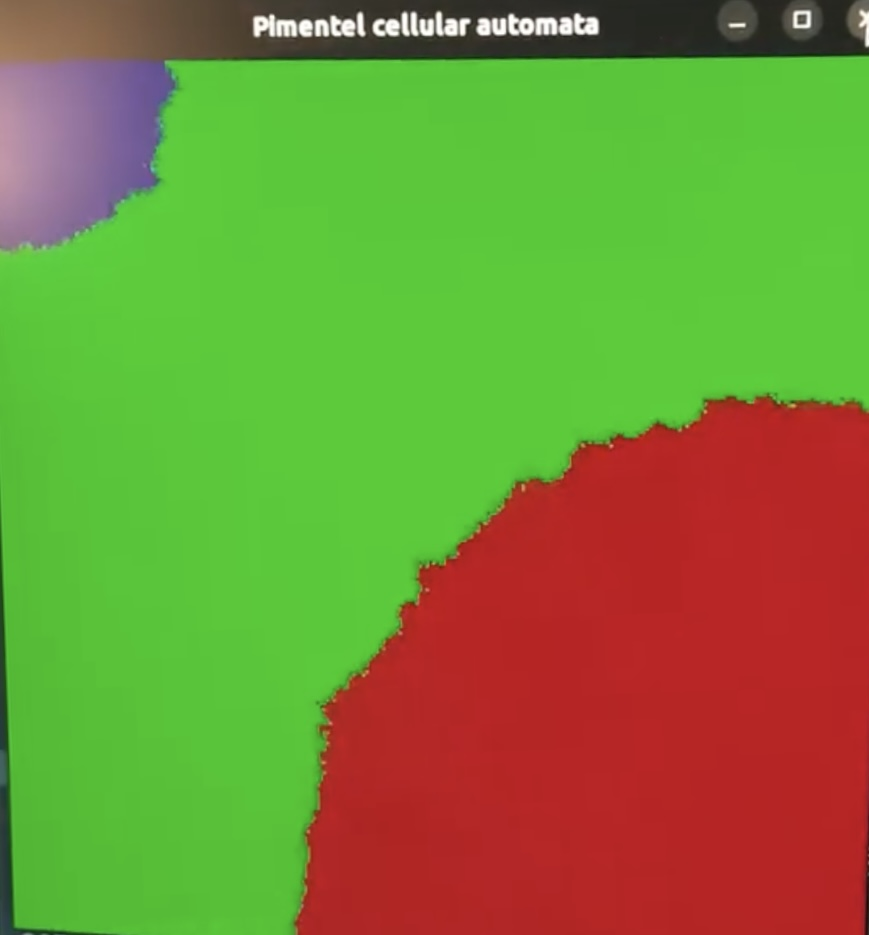
\includegraphics[width=\textwidth]{chapter8/IMG_ch8/pims/pim1.jpg}
    \end{subfigure}
    \hspace{\fill}
    \begin{subfigure}{0.22\textwidth}
        \centering
        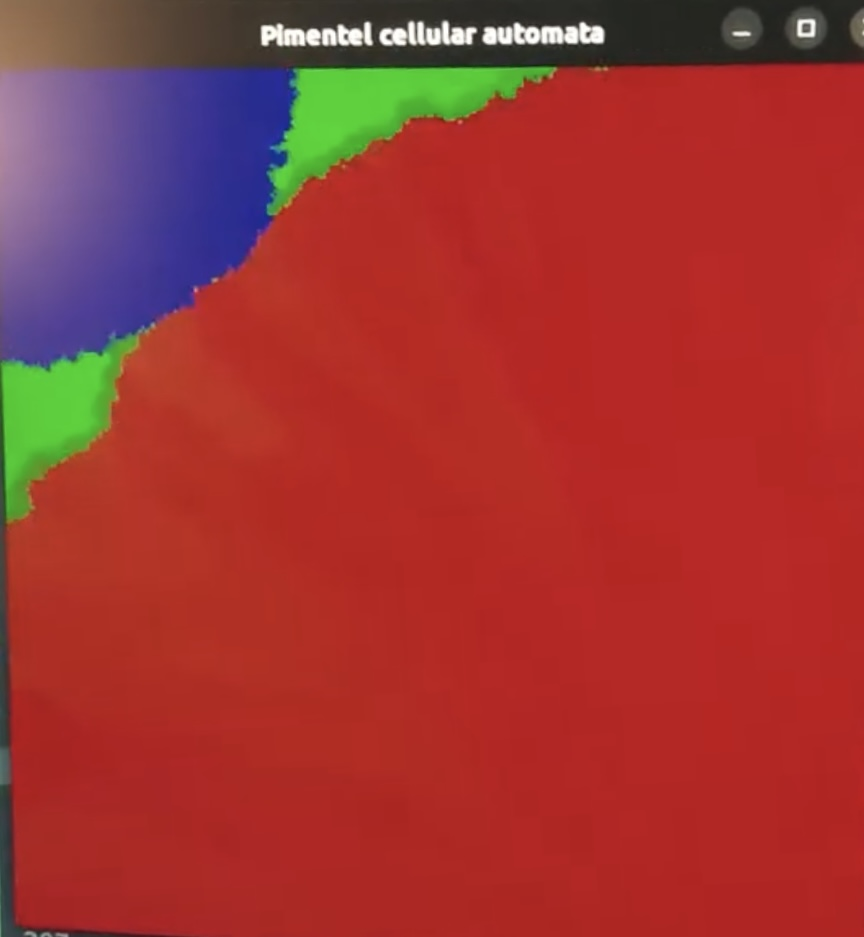
\includegraphics[width=\textwidth]{chapter8/IMG_ch8/pims/pim2.jpg}
    \end{subfigure}
    \hspace{\fill}
    \begin{subfigure}{0.22\textwidth}
        \centering
        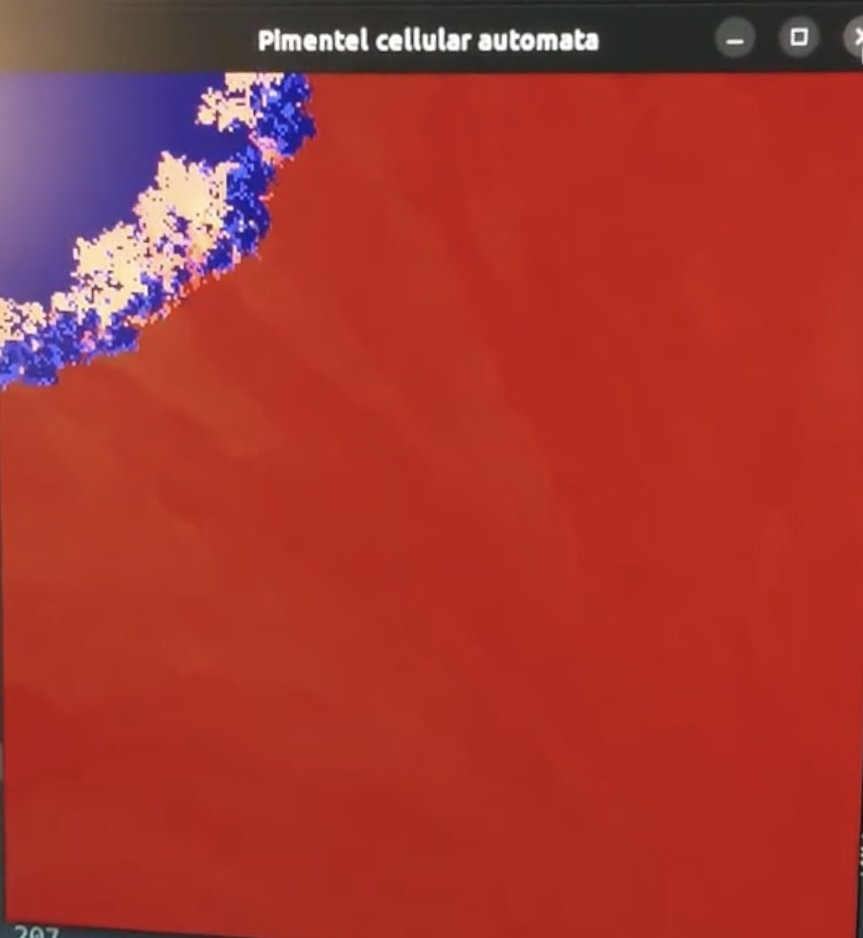
\includegraphics[width=\textwidth]{chapter8/IMG_ch8/pims/pim3.jpg}
    \end{subfigure}
    \hspace{\fill}
    \begin{subfigure}{0.22\textwidth}
        \centering
        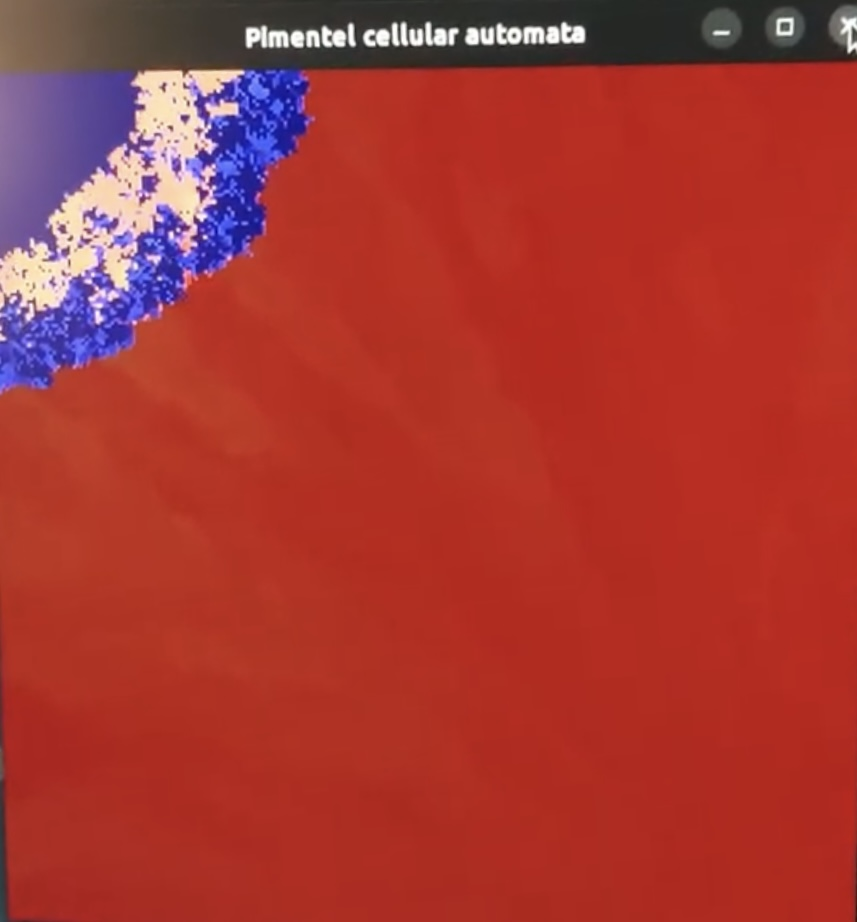
\includegraphics[width=\textwidth]{chapter8/IMG_ch8/pims/pim4.jpg}
    \end{subfigure}
    
    \vspace{0.5em} % Small vertical space between rows

    % Second row of four images
    \begin{subfigure}{0.22\textwidth}
        \centering
        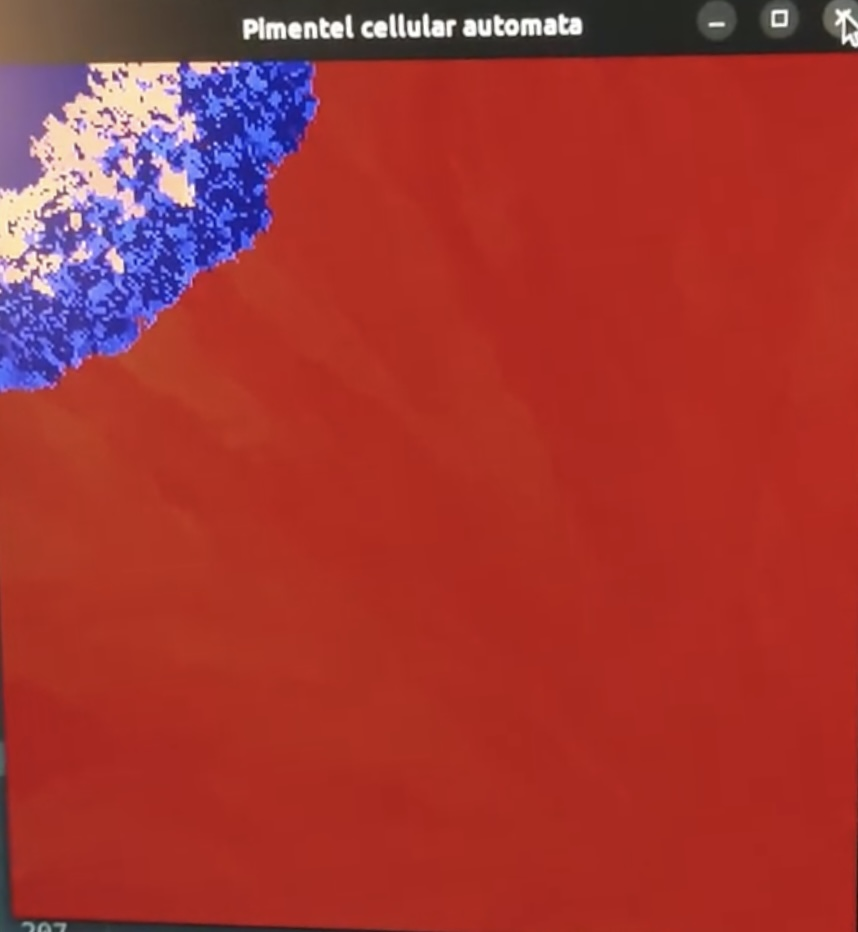
\includegraphics[width=\textwidth]{chapter8/IMG_ch8/pims/pim5.jpg}
    \end{subfigure}
    \hspace{\fill}
    \begin{subfigure}{0.22\textwidth}
        \centering
        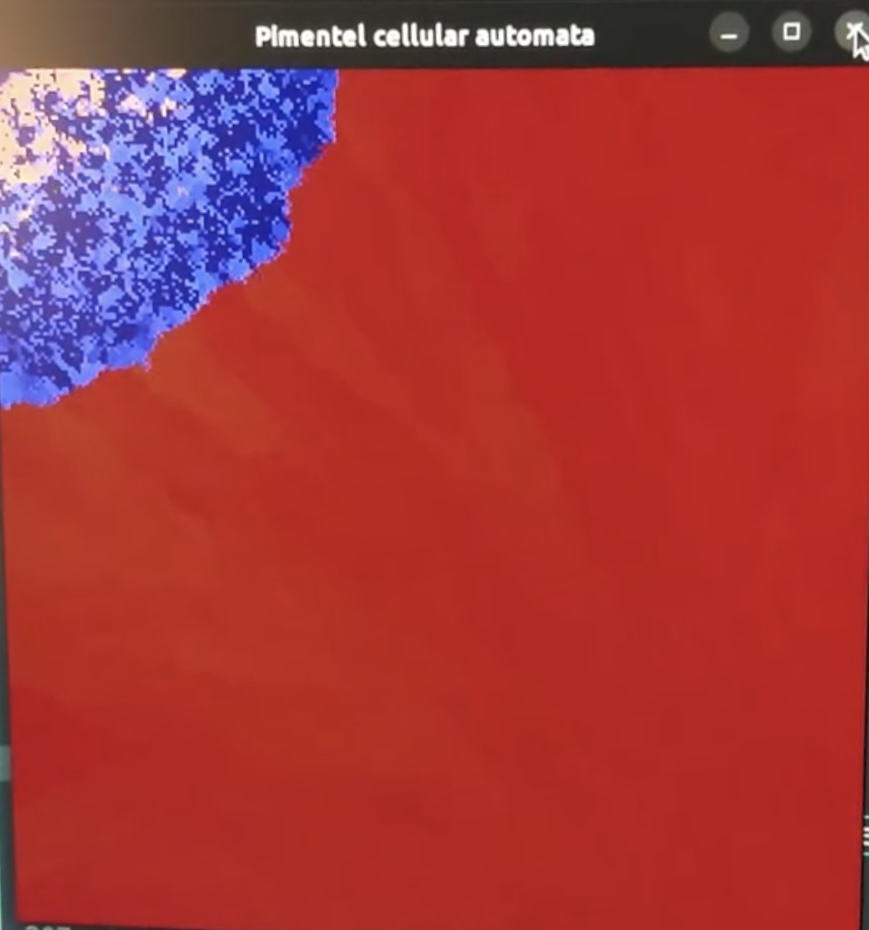
\includegraphics[width=\textwidth]{chapter8/IMG_ch8/pims/pim6.jpg}
    \end{subfigure}
    \hspace{\fill}
    \begin{subfigure}{0.22\textwidth}
        \centering
        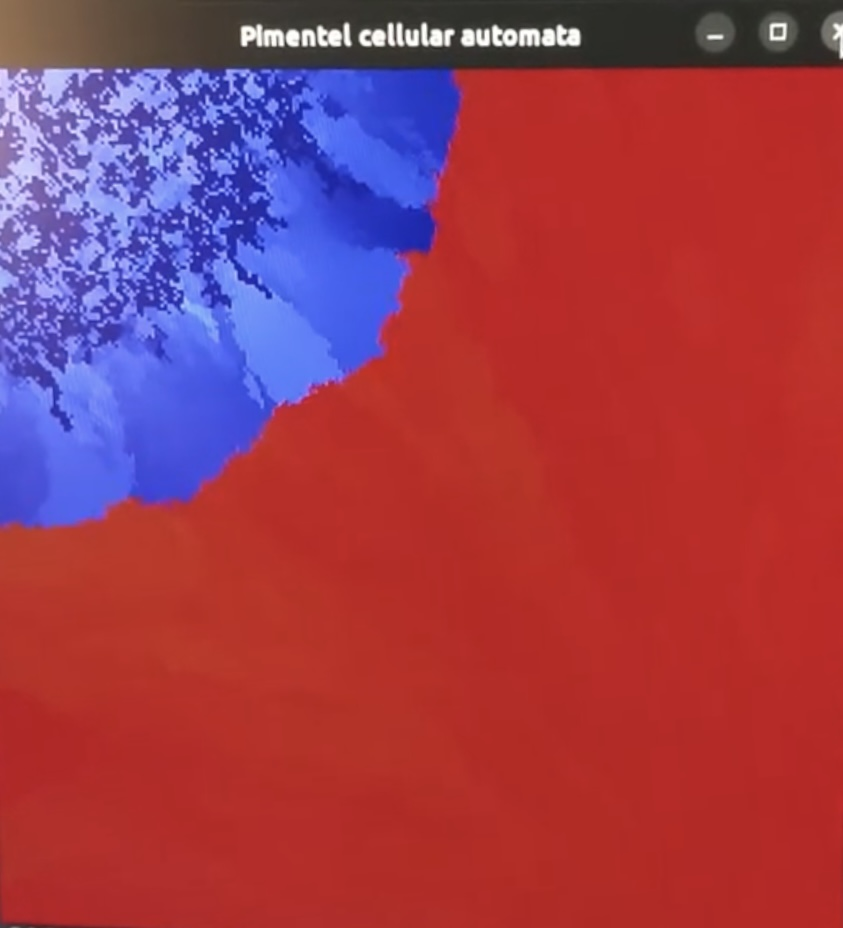
\includegraphics[width=\textwidth]{chapter8/IMG_ch8/pims/pim7.jpg}
    \end{subfigure}
    \hspace{\fill}
    \begin{subfigure}{0.22\textwidth}
        \centering
        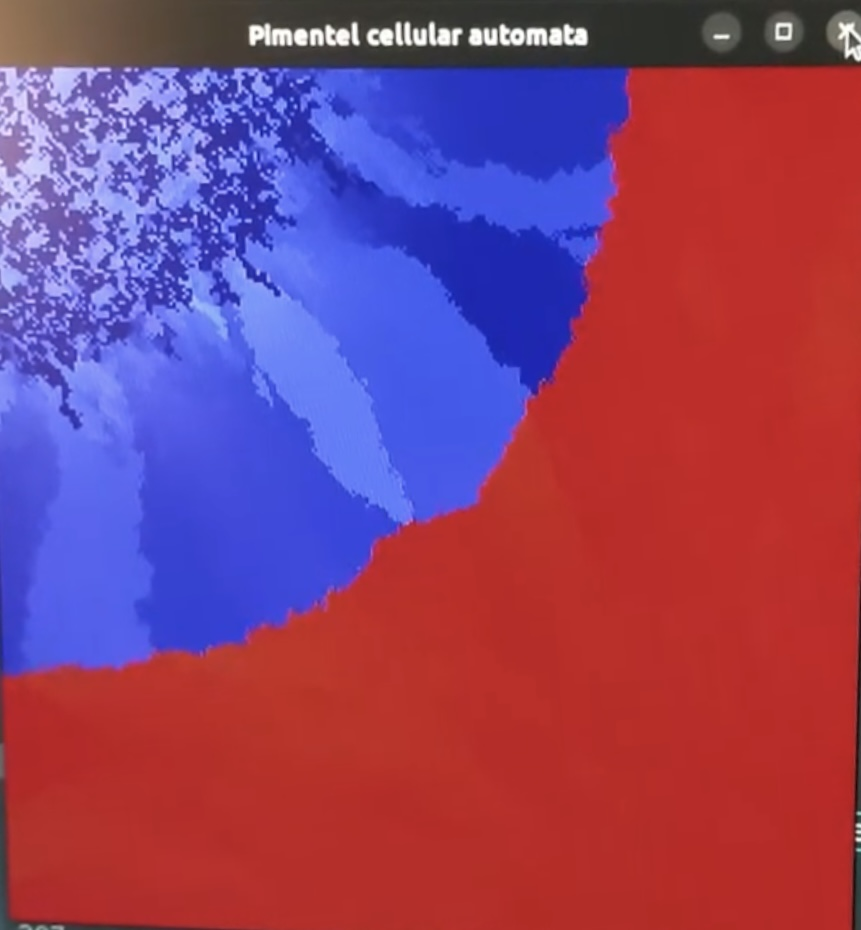
\includegraphics[width=\textwidth]{chapter8/IMG_ch8/pims/pim8.jpg}
    \end{subfigure}

    \vspace{0.5em} % Small vertical space between rows

    % Third row of three images
    \begin{subfigure}{0.22\textwidth}
        \centering
        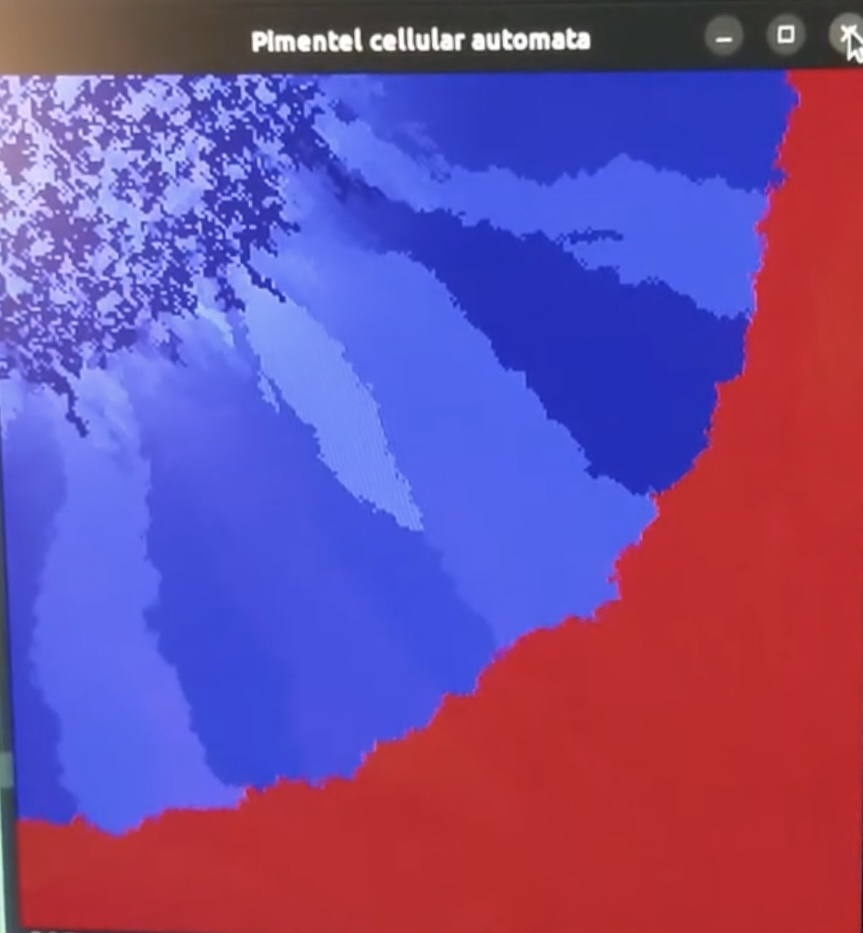
\includegraphics[width=\textwidth]{chapter8/IMG_ch8/pims/pim9.jpg}
    \end{subfigure}
    \hspace{10pt}
    \begin{subfigure}{0.22\textwidth}
        \centering
        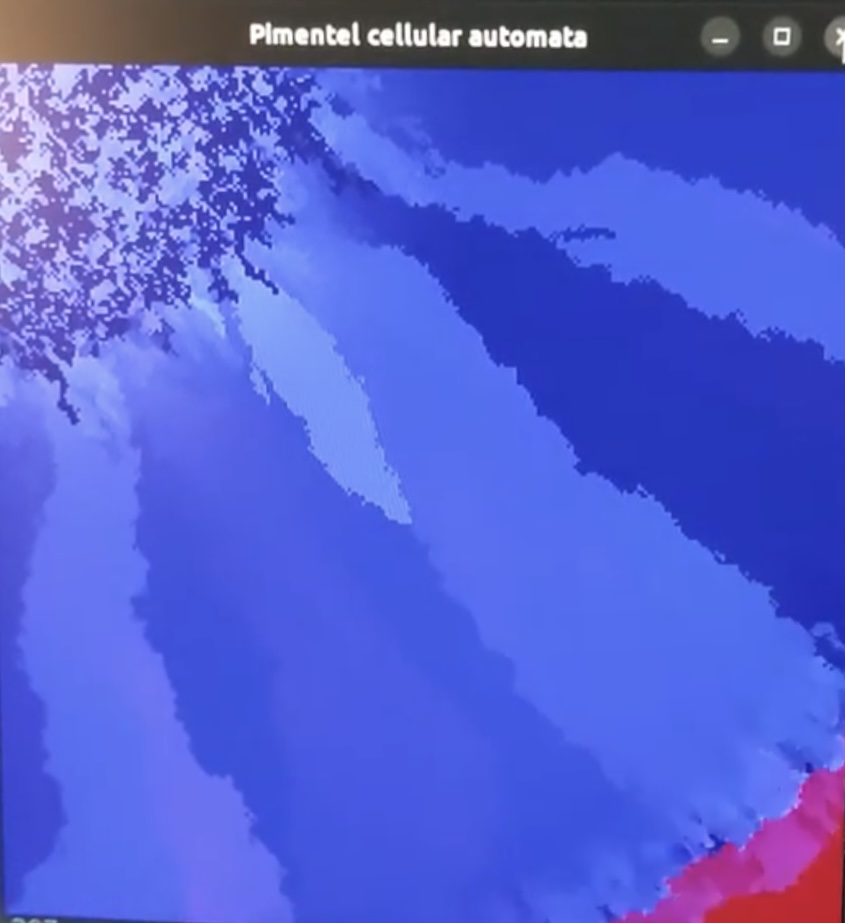
\includegraphics[width=\textwidth]{chapter8/IMG_ch8/pims/pim10.jpg}
    \end{subfigure}
     \hspace{10pt}
    \begin{subfigure}{0.22\textwidth}
        \centering
        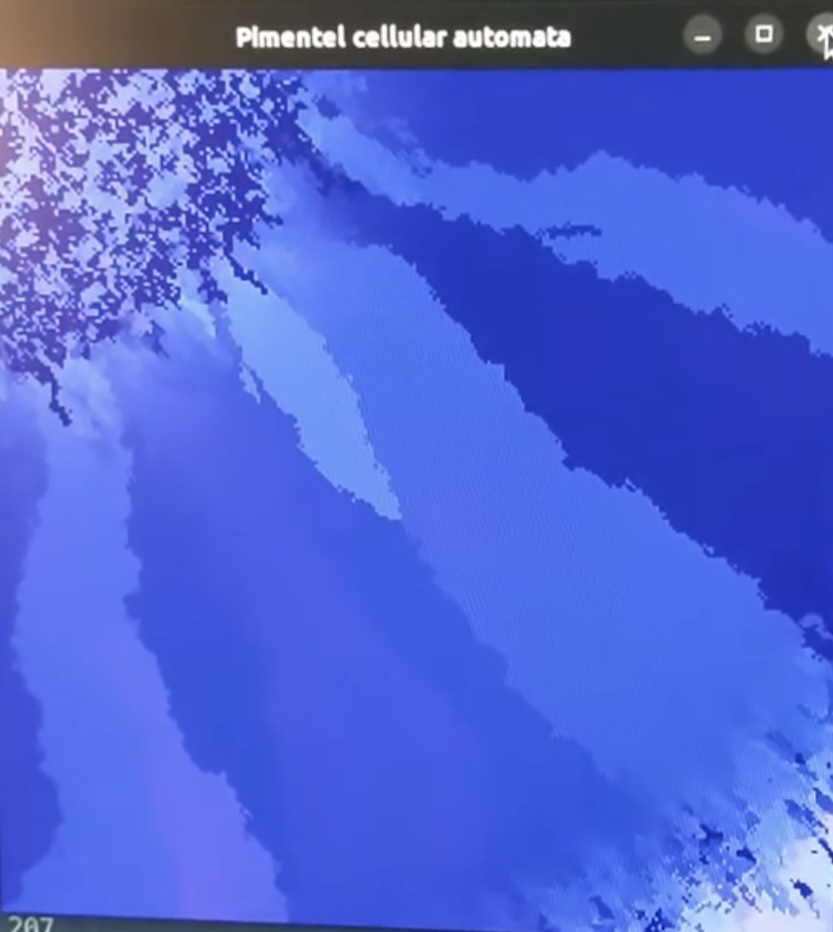
\includegraphics[width=\textwidth]{chapter8/IMG_ch8/pims/pim11.jpg}
    \end{subfigure}

    % Single caption for all images
    \caption{Picured above is a series of frames from an animation: a spatial cellular automaton version of the pimental model. You can see that the initial advantage of the red population is cast aside by the blues after they become hardened and more competetive following intraspecific interactions. The shades within each population only depict relative heredity and don't have any bearing on the dynamics. }
    \label{fig:sequential_images}
\end{figure}











































\subsection{Pimental +}


\noindent
It might be possible to use the pimental model to frame a description of a hypothetical link between speciation and population collapse. An endogeneous process in which the unleasing of variation (facilitated by favourable conditions), can ultimately lead to the demise of a population, as other groups rise to dominance. This process is an attempt to mathematisize what Nietzcche described alegorically in words: the process by which group variation results from favourable circumstances, but how this itself can lead to failiure through a weakining of established forms. The following quote is from``Beyond good and evil'' section 262 \cite{nietzsche2013beyond}:


\begin{quotation}
``A species originates, and a type becomes established and strong in the long struggle with
essentially constant unfavourable conditions. On the other hand, it is known by the experience of
breeders that species which receive super-abundant nourishment, and in general a surplus of
protection and care, immediately tend in the most marked way to develop variations, and are
fertile in prodigies and monstrosities (also in monstrous vices). Now look at an aristocratic
commonwealth, say an ancient Greek polis, or Venice, as a voluntary or involuntary contrivance
for the purpose of rearing human beings; there are there men beside one another, thrown upon
their own resources, who want to make their species prevail, chiefly because they must prevail,
or else run the terrible danger of being exterminated. The favour, the super-abundance, the
protection are there lacking under which variations are fostered; the species needs itself as
species, as something which, precisely by virtue of its hardness, its uniformity, and simplicity of
structure, can in general prevail and make itself permanent in constant struggle with its
neighbours, or with rebellious or rebellion-threatening vassals. The most varied experience
teaches it what are the qualities to which it principally owes the fact that it still exists, in spite of
all Gods and men, and has hitherto been victorious: these qualities it calls virtues, and these
virtues alone it develops to maturity. It does so with severity, indeed it desires severity; every
aristocratic morality is intolerant in the education of youth, in the control of women, in the
marriage customs, in the relations of old and young, in the penal laws (which have an eye only
for the degenerating): it counts intolerance itself among the virtues, under the name of "justice."
A type with few, but very marked features, a species of severe, warlike, wisely silent, reserved,
and reticent men (and as such, with the most delicate sensibility for the charm and nuances of
society) is thus established, unaffected by the vicissitudes of generations; the constant struggle
with uniform unfavourable conditions is, as already remarked, the cause of a type becoming
stable and hard. Finally, however, a happy state of things results, the enormous tension is
relaxed; there are perhaps no more enemies among the neighbouring peoples, and the means of
life, even of the enjoyment of life, are present in super abundance. With one stroke the bond and
constraint of the old discipline severs: it is no longer regarded as necessary, as a condition of
existence--if it would continue, it can only do so as a form of luxury, as an archaising taste.
Variations, whether they be deviations (into the higher, finer, and rarer), or deteriorations and
monstrosities, appear suddenly on the scene in the greatest exuberance and splendour; the
individual dares to be individual and detach himself. At this turning-point of history there
manifest themselves, side by side, and often mixed and entangled together, a magnificent,
manifold, virgin-forest-like up-growth and up-striving, a kind of tropical tempo in the rivalry of
growth, and an extraordinary decay and self-destruction, owing to the savagely opposing and
seemingly exploding egoisms, which strive with one an other "for sun and light," and can no
longer assign any limit, restraint, or forbearance for themselves by means of the hitherto existing
morality. It was this morality itself which piled up the strength so enormously, which bent the
bow in so threatening a manner:--it is now "out of date," it is getting "out of date." The
dangerous and disquieting point has been reached when the greater, more manifold, more
comprehensive life is lived beyond the old morality; the "individual" stands out, and is obliged to
have recourse to his own law-giving, his own arts and artifices for self-preservation, self-
elevation, and self-deliverance. Nothing but new "Whys," nothing but new "Hows," no common
formulas any longer, misunderstanding and disregard in league with each other, decay,
deterioration, and the loftiest desires frightfully entangled, the genius of the race overflowing
from all the cornucopias of good and bad, a portentous simultaneousness of Spring and Autumn,
full of new charms and mysteries peculiar to the fresh, still inexhausted, still unwearied
corruption. Danger is again present, the mother of morality, great danger; this time shifted into
the individual, into the neighbour and friend, into the street, into their own child, into their own
heart, into all the most personal and secret recesses of their desires and volitions. What will the
moral philosophers who appear at this time have to preach? They discover, these sharp onlookers
and loafers, that the end is quickly approaching, that everything around them decays and
produces decay, that nothing will endure until the day after to-morrow, except one species of
man, the incurably mediocre. The mediocre alone have a prospect of continuing and propagating
themselves--they will be the men of the future, the sole survivors; "be like them! become
mediocre!" is now the only morality which has still a significance, which still obtains a hearing.--
But it is difficult to preach this morality of mediocrity! it can never avow what it is and what it
desires! it has to talk of moderation and dignity and duty and brotherly love--it will have
difficulty in concealing its irony!''
\end{quotation}

The basic pimental model as defined above encorporates the fitness of two populations, these increasing when the particular species is pushed into a minority. 

$$\pr{\Delta A_t = 1} = \frac{A_t}{N} \frac{f_a}{\bar f}$$

$$\pr{\Delta A_t = 1} =\lrb{ 1 - \frac{A_t}{N}} \frac{f_b}{\bar f}$$




where $A_t$, $B_t$, and $N$ represent the relative domination of group $A$, group $B$, and the total domain capacity. With the Moran assumption, $A_t = N - B_t$. Like above, these are essentially the probabilities of a chosen individual encountering a member of the opposite group ($A_t/N$) \textbf{and} defeating them in competition ${f_a}/{\bar f}$. In this unaltered model, fitness changes according to

$$f_a(t+\Delta t) = f_a(t) + \delta \lrb{\frac{B_t}{A_t}}^\alpha$$

$$f_b(t+\Delta t) = f_b(t) + \delta \lrb{\frac{A_t}{B_t}}^\alpha$$

\noindent
Note: this is a slightly different definition to the one shown above. $R_a$ \& $R_b$ are replaced by $f_a$ \& $f_b$, but the dynamics are at least qualitativaly identical. 

\subsubsection*{Sub-species, including variable speciaton}

Suppose we incorporate a species count for each population, $\xt^{(a)}$ and $\xt^{(b)}$, respectively. According to the alagory laid out by neitche, exxessive variation (the emergence of many species), leads to a weakening of a population. In our model, that would be represented by a drop in fittness. But how does the number of species change. Generally speaking, variation will increase when the demands of survival are lessened by favourable circumstances. In our model, something like this will be represented by the product of domain control and fitness.\par 
Take for example

$$\pr{\Delta \xt^{(a)} = 1}  = \beta_a\xt^{(a)} \Delta t$$

$$\pr{\Delta \xt^{(a)} = -1}  = \mu_a\xt^{(a)} \Delta t$$

\noindent
with extinction $\mu_a$ constant, and speciation $\beta_a$ varing according to fitness, $f_a$, and relative domination $(A_t / N)$:

$$\beta_a = \lrb{\frac{A_t}{N}}^\lambda f_a$$ 

\noindent
The dynamics for the other species count $\xt^{(b)}$ would function in the same way but with $A_t$ being replaced by $B_t$ etc... 

\subsubsection*{Effect of species count on fitness}

\noindent
Then there is the effect of excess variation on reducing a group's fitness.Something like this could serve well,

$$f_a(t+\Delta t) = f_a(t) + \delta \lrb{\frac{B_t}{A_t}}^\alpha  - \gamma \xt^{(a)}$$

$$f_b(t+\Delta t) = f_b(t) + \delta \lrb{\frac{A_t}{B_t}}^\alpha  - \gamma \xt^{(b)}$$

\noindent
with constant $\gamma$ representing the abount by which the inneficencies of excess variations weigh on overall performance. \par 

\subsubsection*{Comments}
Unfortunately, for this model, along with half a dozen other speculative models relating to speciation and evolution, I didn't get round to running simulations or doing much analysis. This is inevitable. and the model outlined here is itself a description of why. Models, like any other form of coded information are subject to the laws of variation whereby one model, on creative consideration, soon gives birth to many more. And with time and energy resources being limited, a multiplicity like this hs the effect of spreading resources more thinly, each gets less and less attention as the number increases. And before you know it, its time to write a thesis, and most of them get discarded.\par
But I thought, I'd at least write this one down, because it contains my best attempt at describing mathematically the endogeneous aspect of collapse by variation.  


















\section{Allegorical model of rise run ruin rejuvenation}


I wanted to try to represent a certain style of stochastic cyclic dynamics. A pattern in which potential (energy) builds up constantly in the absence of use.  Then in surplus, the count of individual agencies (species) increases in response to the excessive energy potential. \par 
The potential is diminished by the large number of agencies until at some time,  a state of scarcity comes about. And in this, there is a catastrophic extinction in which all of the agencies die. In reality, not all of the agencies (species) will die, some will remain and become distinct in the newly hash selective conditions. \par 
From here, the cycle repeats. Potential once more begins to build until a Poission revival kickes off a new proliferative wave.  Yes, in reality, this will begin from one or a few of the agencies  remaining beyond the catastrophe. \par




\noindent
The purpose of this model is to make some link between a potential dynamics in the cyclic rise and decline of dissipative structures in the context of a constant supply of energy.  We perhaps see this style of dynamics both in the cyclic dynamics of turbulance shedding in the Stokes flow around a circle, and the periodic rise and collapse of ecosystems and even cultures. 

\subsection*{Model specification}

% Just notes, not final

(Energy availability)
 $$\ddt{N} = \xi - \mu \xt$$
(Segregation into multiplicity)
$$\pr{\Delta \xt = 1} = \lambda \xt \delt + o(\delt)$$
(Catastrophic collapse)
$$\pr{\xdt = 0 | \xt} =  \delta \frac{\xt}{N(t)} \delt +o(\delt)$$
(Poisson revival)
$$\pr{\xdt = 1 | \xt = 0} = \alpha \delt + o(\delt)$$
(No event)
$$\pr{\xdt = \xt} = 1 - \lrb{\lambda \xt  + \delta \frac{\xt}{N(t)} + \alpha   }\delt + o(\delt)$$





\begin{figure}[H]
    \centering
    % First figure
    \begin{subfigure}{0.48\textwidth}
        \centering
        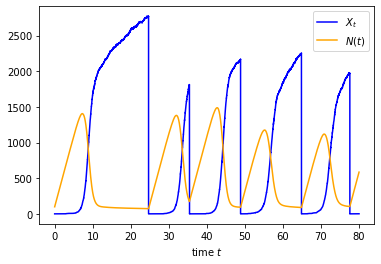
\includegraphics[width=\textwidth]{chapter8/IMG_ch8/VBCfigs/80for1VBC} % Adjust the image path as necessary
    \end{subfigure}
    \hspace{\fill} % Optional: adds space between figures
    % Second figure
    \begin{subfigure}{0.48\textwidth}
        \centering
        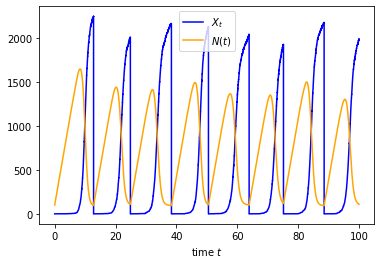
\includegraphics[width=\textwidth]{chapter8/IMG_ch8/VBCfigs/100for1VBC} % Adjust the image path as necessary
    \end{subfigure}
    
    \caption{Realisations of the model.  Potential energy, $N(t)$,  shown in orange, agency count,  $\xt$, in blue.}
    \label{fig:two_figures}
\end{figure}



\begin{figure}[H]
    \centering
    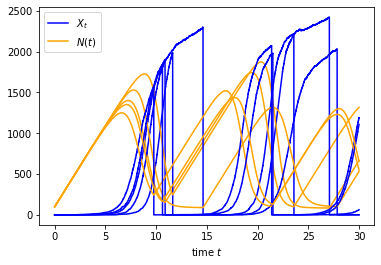
\includegraphics[width=0.7\textwidth]{chapter8/IMG_ch8/VBCfigs/30for5VBC} % Adjust the width as needed
    \caption{Multiple realisations with the same parameters and initial condition.}
    \label{fig:single_figure}
\end{figure}









\noindent
$\xt$, the replicative units (or objects of multiplicity in segregation) can be thought to represent a great many different things. They may be framed as the individuals in a population; of bacteria, viruses, organisms. They may be species within a genre, fractured but internally coherent groups within a broader population. Autonomous agencies within an organisation --- this is quite a general concept and could be applied to a number of situations: teams in a company, parties in a political system. A great many things can be placed in these terms... It would be fair to say that some of these representations are loose and ill-defined. But there is a more general way of looking at it, at what the quantity $\xt$ is attempting to capture. It's a proxy for order. That is, negative entropy. Think for a moment of a further analogy in fluid flows. If we observe the transition form laminar flow to turbulence, there is a fragmenting of flow directions. At first, all streamlines point in one onwards direction of motion. At the end of the transition, there are what appears to be an infinitude of ever more minute and fleeting divergences; of flow-lines separating off from one-another.\par



Admittedly, this does happen in spatial continuum rather than discrete jumps. But say for a moment we were to view this degenerative separation at a course grain. We might see from the outset an initial branching into two distinct pathways. Each of which encompassing fluid flow of roughly coherent direction. Each of these then has the potential to further subdivide into two. And each time this breakage takes place, there is further dissipation. In our coarse approximate description, there are a greater number of flow interfaces --- more locations of friction. Each sub-stream, smaller and smaller in cross-section will carry less and less kinetic energy and a greater proportion of the energy will be lost as heat.\par 
Towards the limit, minute, infinitely multiplicitous and scattered fluid trajectories will become so energy lacking as to resemble little more than stationary fluid. 
From here, with ongoing general flow, there will be a re-cohering into a more broadly aligned fluid stream. This, then, will likely be seen to once more progress in a dissipative turbulent divergence as before. In this way, a kind of oscillation commences. From Laminar, to turbulent, and through fizzling out, back to laminar, turbulent, so on and so forth. 

In real fluid flows --- take for example flow around a circle (or sphere in three dimensions) --- the oscillation is not absolute; both more turbulent and less turbulent regions coexist in an oscillatory spatial continuum. Laminar flow begins to shed turbulence as it sways one way in the wake of the circle; then going on to drift back into where the turbulence last was.\par 


Let us turn to another example of a dissipative structure: the fragmenting of a genus population into species over large swathes of time. That this is an example of a Prigoginian dissipative structure is a claim worth scrutinizing. I do believe it has been made before by others \cite{elitzur1994let} \cite{sharma2023assembly}.  None the less, let us be careful. 

Living organisms are one of the most rapidly dissipating arrangements in the universe. It has been observed that per kilogram, humans and other terrestrial life forms dissipate energy as a rate orders of magnitude greater than the sun. They are also highly ordered, local low-entropy formations which are kept far above equilibrium by their continual usage of energy. So it seems natural to assign the term ``dissipative structure'' to living organisms taken at the individual level. 
But can we speak more generally about life and its natural progressions? Over time, genera fragment into species. It seems straightforward that this is an example of entropy reduction.  



\vspace{10pt}

\hrule

\vspace{10pt}



\noindent
\textbf{Aside:} In "The genetical theory of natural selection" (1930),  R.  Fisher makes mentions something in relation to this line of thought: 

\begin{quote}
\noindent
"A philospohical view of history, which has attained to great popularity in several continental countries,  regards the rise as well as the fall of civilisations as but successive phases of a cycle of growth and decay,  which, it is supposed, repeats itself endlessly,  throughout human history.  So long as we aim at no more than an effective generalised description of the phenomena there is much to be said for considering the phases of rise and development of the great civilisations in conjunction with the phases of their decayand collapse. It is a real advantage that the parallelisms between the earlier phases of different cultures should be recognised, and that their relations in time to recognizably parallel later phases should be established as accurately as possible.  Generalised description should, however,  never be regarded as an aim in itself."
\end{quote}

"Generalised description should, however,  never be regarded as an aim in itself" -- maybe I should have read this before working on the equations above.  But perhaps there is a certain utility in the aesthetic of a generalised description when it becomes codified in the language of a mathematical model. 




\vspace{10pt}

\hrule


\vspace{10pt}





\section*{Bardo Thodol}

 In the Bardo Thodol (otherwise known as The Tibetan book of living and dying), there are listed 6 bardo states which describe the stages of life and the process of transition between lives:

\begin{itemize} \item the bardo of birth \item the bardo of dreams \item the bardo of samadhi meditation \item the bardo of the moment before death \item the bardo of dharmata (pure reality) \item the bardo of becoming \end{itemize}

I can't help but notice a crossover with the first three of these and the stages of the Mandukya Upanishad: A, U, and M for "beginning," "process," and "cessation." This links loosely with the stages of the logistic growth model. Initially, the number of species rapidly increases, then there is a stabilizing phase, and eventually, many die out, leaving only a few. But this is an aside.

The point of the Bardo Thodol demonstrates an understanding of something also revealed by stochastic process theory: that in life, there are periods of relative stasis punctuated by times of great upheaval, change, and above all, uncertainty. The book is a guide for those dying, so that they may pass through the crucial final three stages to attain a favorable passage through the period of undetermined futures. The idea is that their consciousness somehow persists after their physical body dies. It then wanders through the bardo of dharmata, before stumbling upon a series of lights. Each light encountered corresponds to one of the 6 realms of samsara in which the person might find themselves born.

\vspace{5pt} \hrule \vspace{5pt}

\noindent \textbf{Aside -- the 6 realms of samsara: } In Tibetan Buddhist theory, there are 6 "realms" in which all beings supposedly occupy, cycling among them over a series of cycles of birth, death, and rebirth:

\begin{itemize} \item Hell realm(s) \item Animal realm \item Realm of hungry ghosts \item Human realm \item Realm of the jealous gods \item Deva realm \end{itemize}

The stated ideal is to, as it were, exit this process of cycles and become "enlightened." This can only happen at the time of death and supposedly is most easily accomplished when exiting the human realm. The trick is to use the opportunity of non-fixation to remain in the state of transience without falling back into one of the realms, and it is this which the Bardo Thodol aims to guide its recipients towards.

\vspace{5pt} \hrule \vspace{5pt}

The lights seem to be analogous to circumstances that seem appealing but end up as "basins of attraction," whereby entry inevitably leads to an absorption and fixation in that particular realm. There is a clear analogy to observations in stochastic process analysis. For example, at a state of undetermined instability (as in the squeezes that take place when one population is very small in the Pimental model), nearby trajectories diverge as a result of an amplification in the importance of small, otherwise insignificant, stochastic influences.

In this framework, when a person dies, their fated trajectory is yet undecided, and in this state of undetermined instability, small influences can be applied to steer things one way or the other.

\subsubsection*{Why do we care?} In the modern scientific age we live in, most educated people balk and sneer at the concept of life after death.  There appears two angles through which to address the matter:

\begin{itemize} \item \textbf{You could say that there are many lives within one life}, and that the transition between phases of life shares qualities with the stated transition between the bardo of the moment before death and the bardo of becoming. In a way, I feel as if I am embarking on the bardo of the moment before death.  The path of life after a PhD, without concrete plans, can be underermined and subject to an array of possible continuations. 

\item (More abstractly) \textbf{Multiple successive individual people can occupy the same character.} It can be imagined that this effect will have been all the more pronounced in 9th-century Tibet. For centuries, over countless generations, families will have occupied the Tibetan plateau in relative isolation. With this slowed movement, it seems only natural that the perception of rise, fall, and change will have been extended to perceive the agencies living over multiple generations. Take as a prime example the "character" of the Dalai Lama and the continuously reincarnated lamas of the other major schools: one personality, living over 10 or more generations.

New head lamas are selected at birth. They are identified by the elders of the school to be the "reincarnation" of the previous leader. It strikes me as a remarkable mechanism of government for creating piety and meritous behaviour amongst a people: give everyone's child the prospect of becoming leader of the state.

\end{itemize}

\subsection*{Quasistationarity} 

Verging a bit into the reckless and speculative here.  But is there not a philosophical analogy between quasistationarity --- that is,  quantified behaviour of a stochastic process given non-fixation --- and the theoretical description of liberation in the conception of the Bardo Thodol. \par 
Not getting stuck in one of the basins of attraction of the 6 realms, appears similar to not getting stuck, either by depletion to 0 or by catastrophic fixation in the birth death catastrophe process.  Similar to Icarus, neither flying too high or too low,  the liberatee of the bardo of dharmata doesn't get too close to any of the appealing absorbative attractions which would inevitably lead to a re-binding into one of the cyclic domains of samsara.  \par 
Behavior conditional on non-fixation, non rebirth --- that being the practive of the Arahant as that of the Bodisatva.  Unbound and unmarred by conditions of suffering which arise from the succeptability of craving for material manifestations. \par 





\begin{figure}[H] 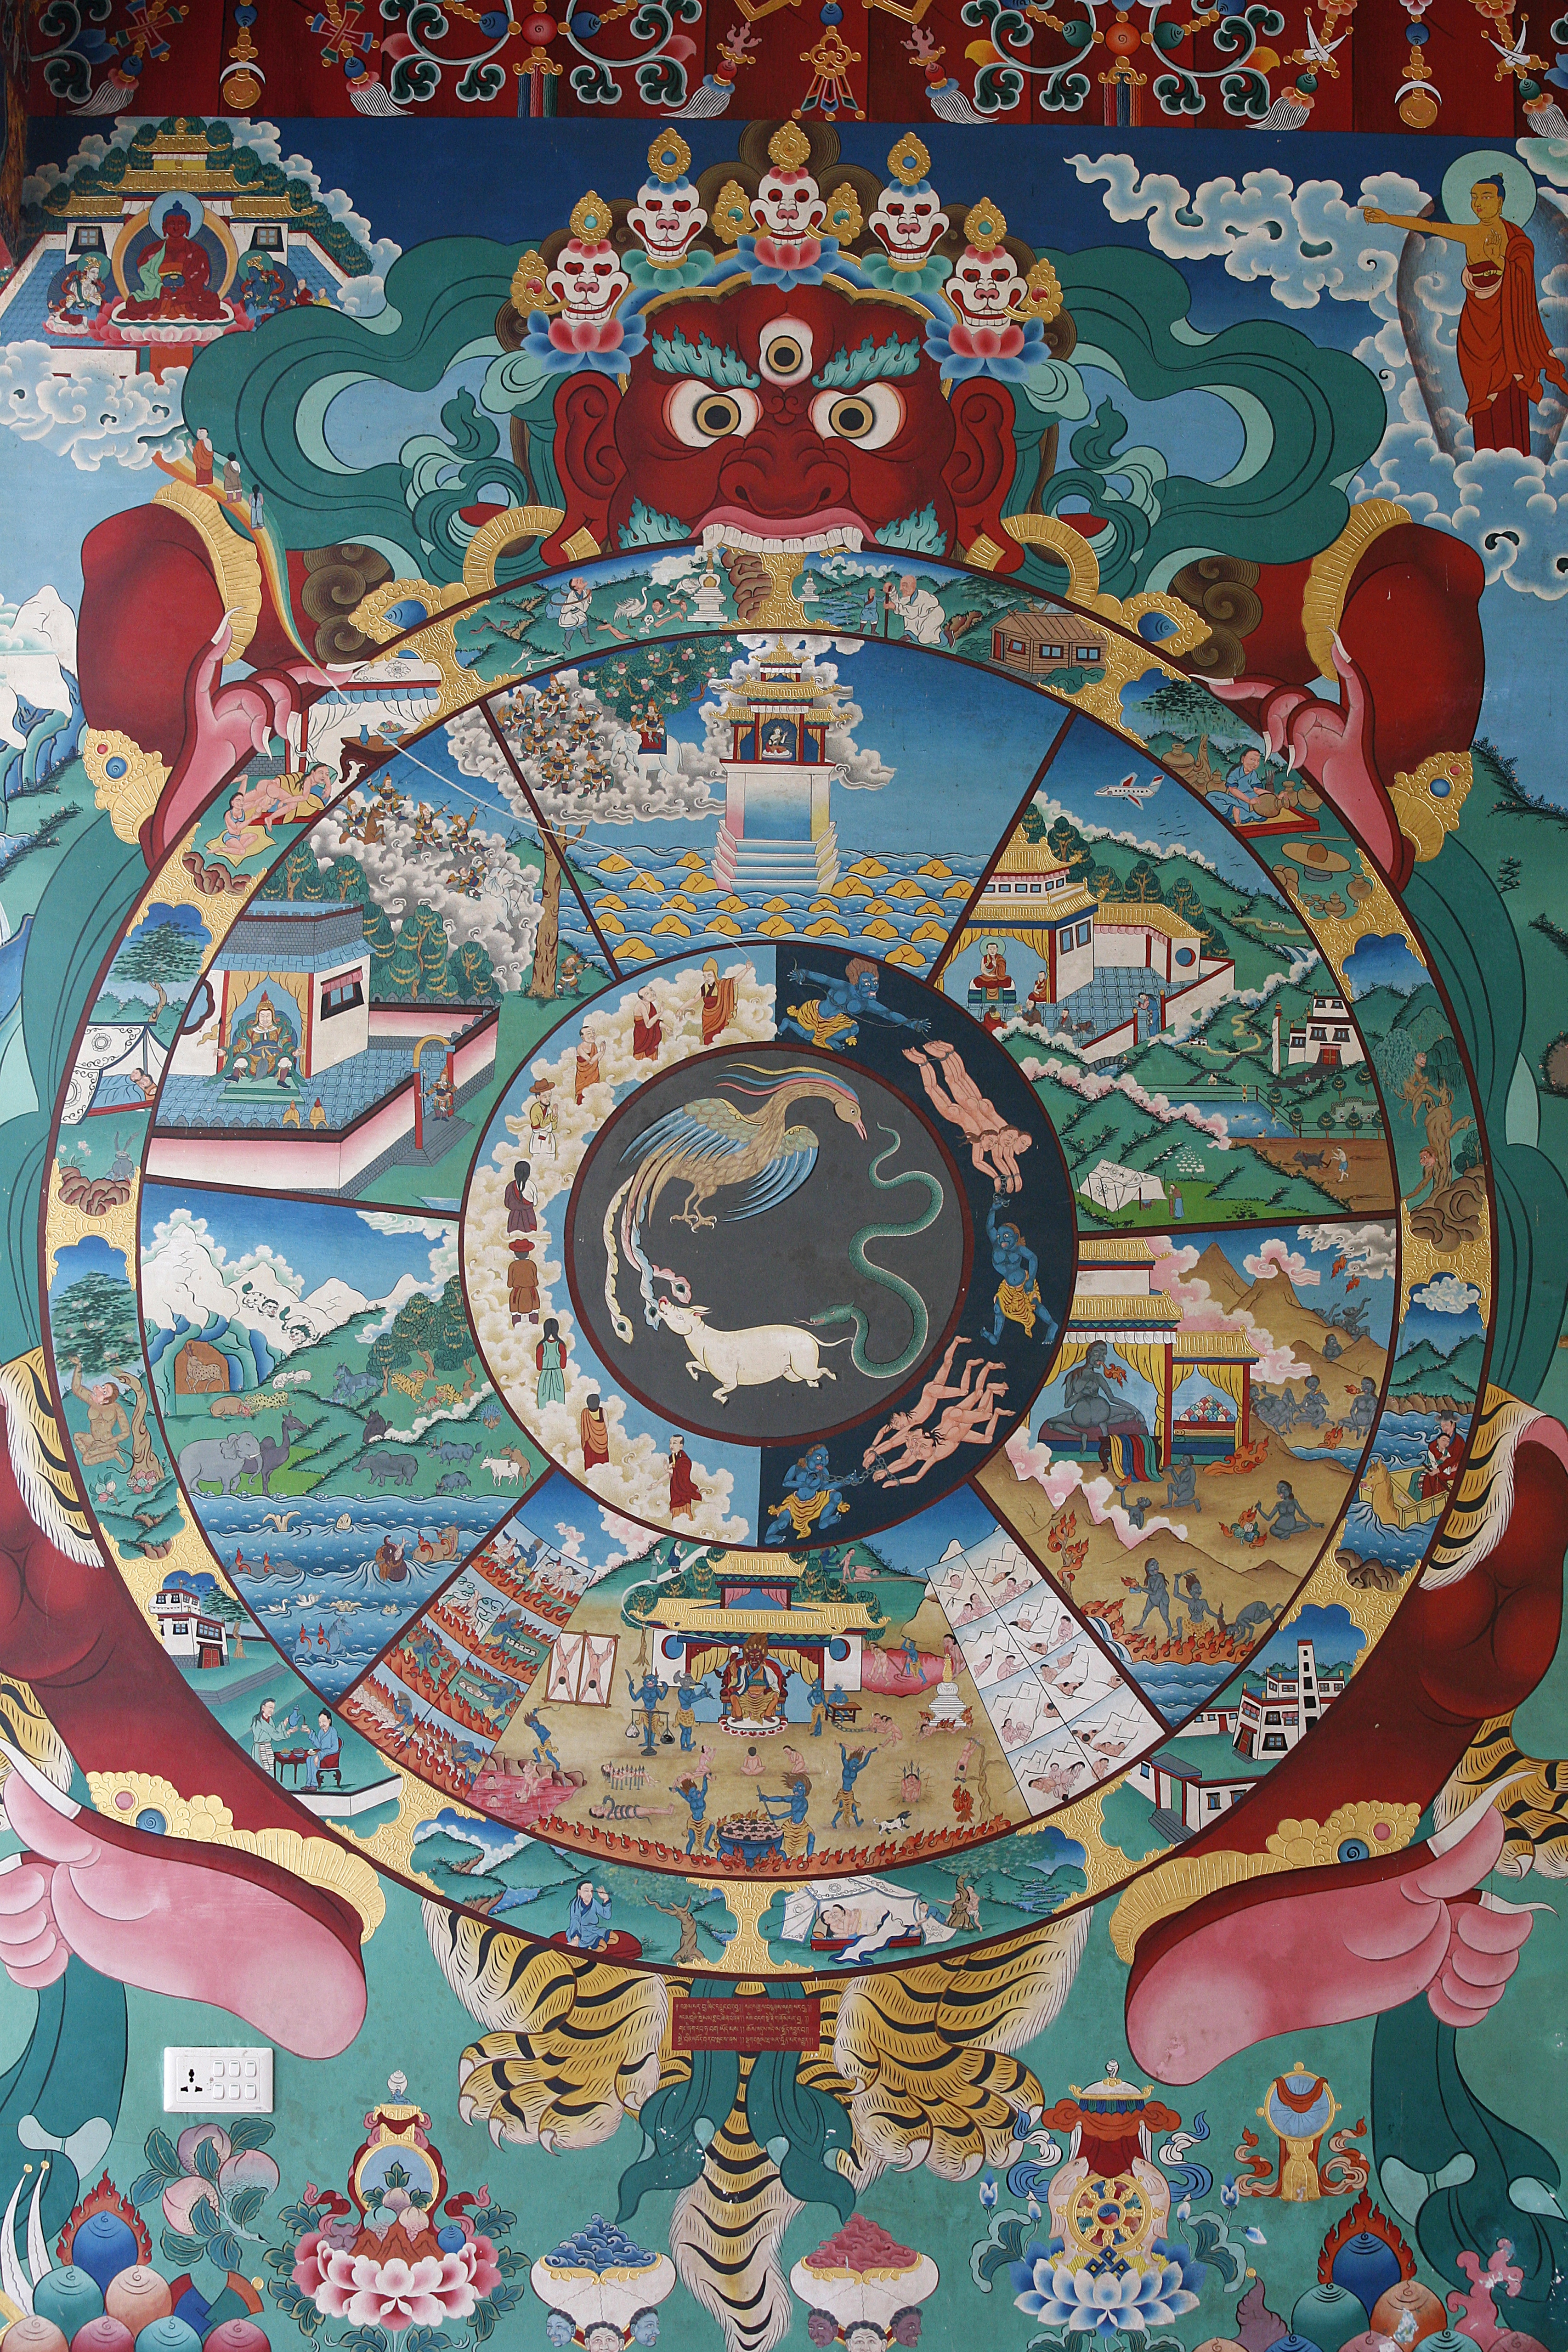
\includegraphics[width = 0.85\textwidth]{chapter8/IMG_ch8/samsara.jpg}
\centering
\pagebreak \caption{Wheel of samsara. Yama (god of death) depicted holding a wheel containing the 6 realms. From the center, a rooster, snake, and pig are shown to represent attachment, aversion, and ignorance respectively. They are said to link with one another cyclically, causing the dynamism which makes the wheel progress.} \label{redone} \end{figure}

\begin{figure}[H] 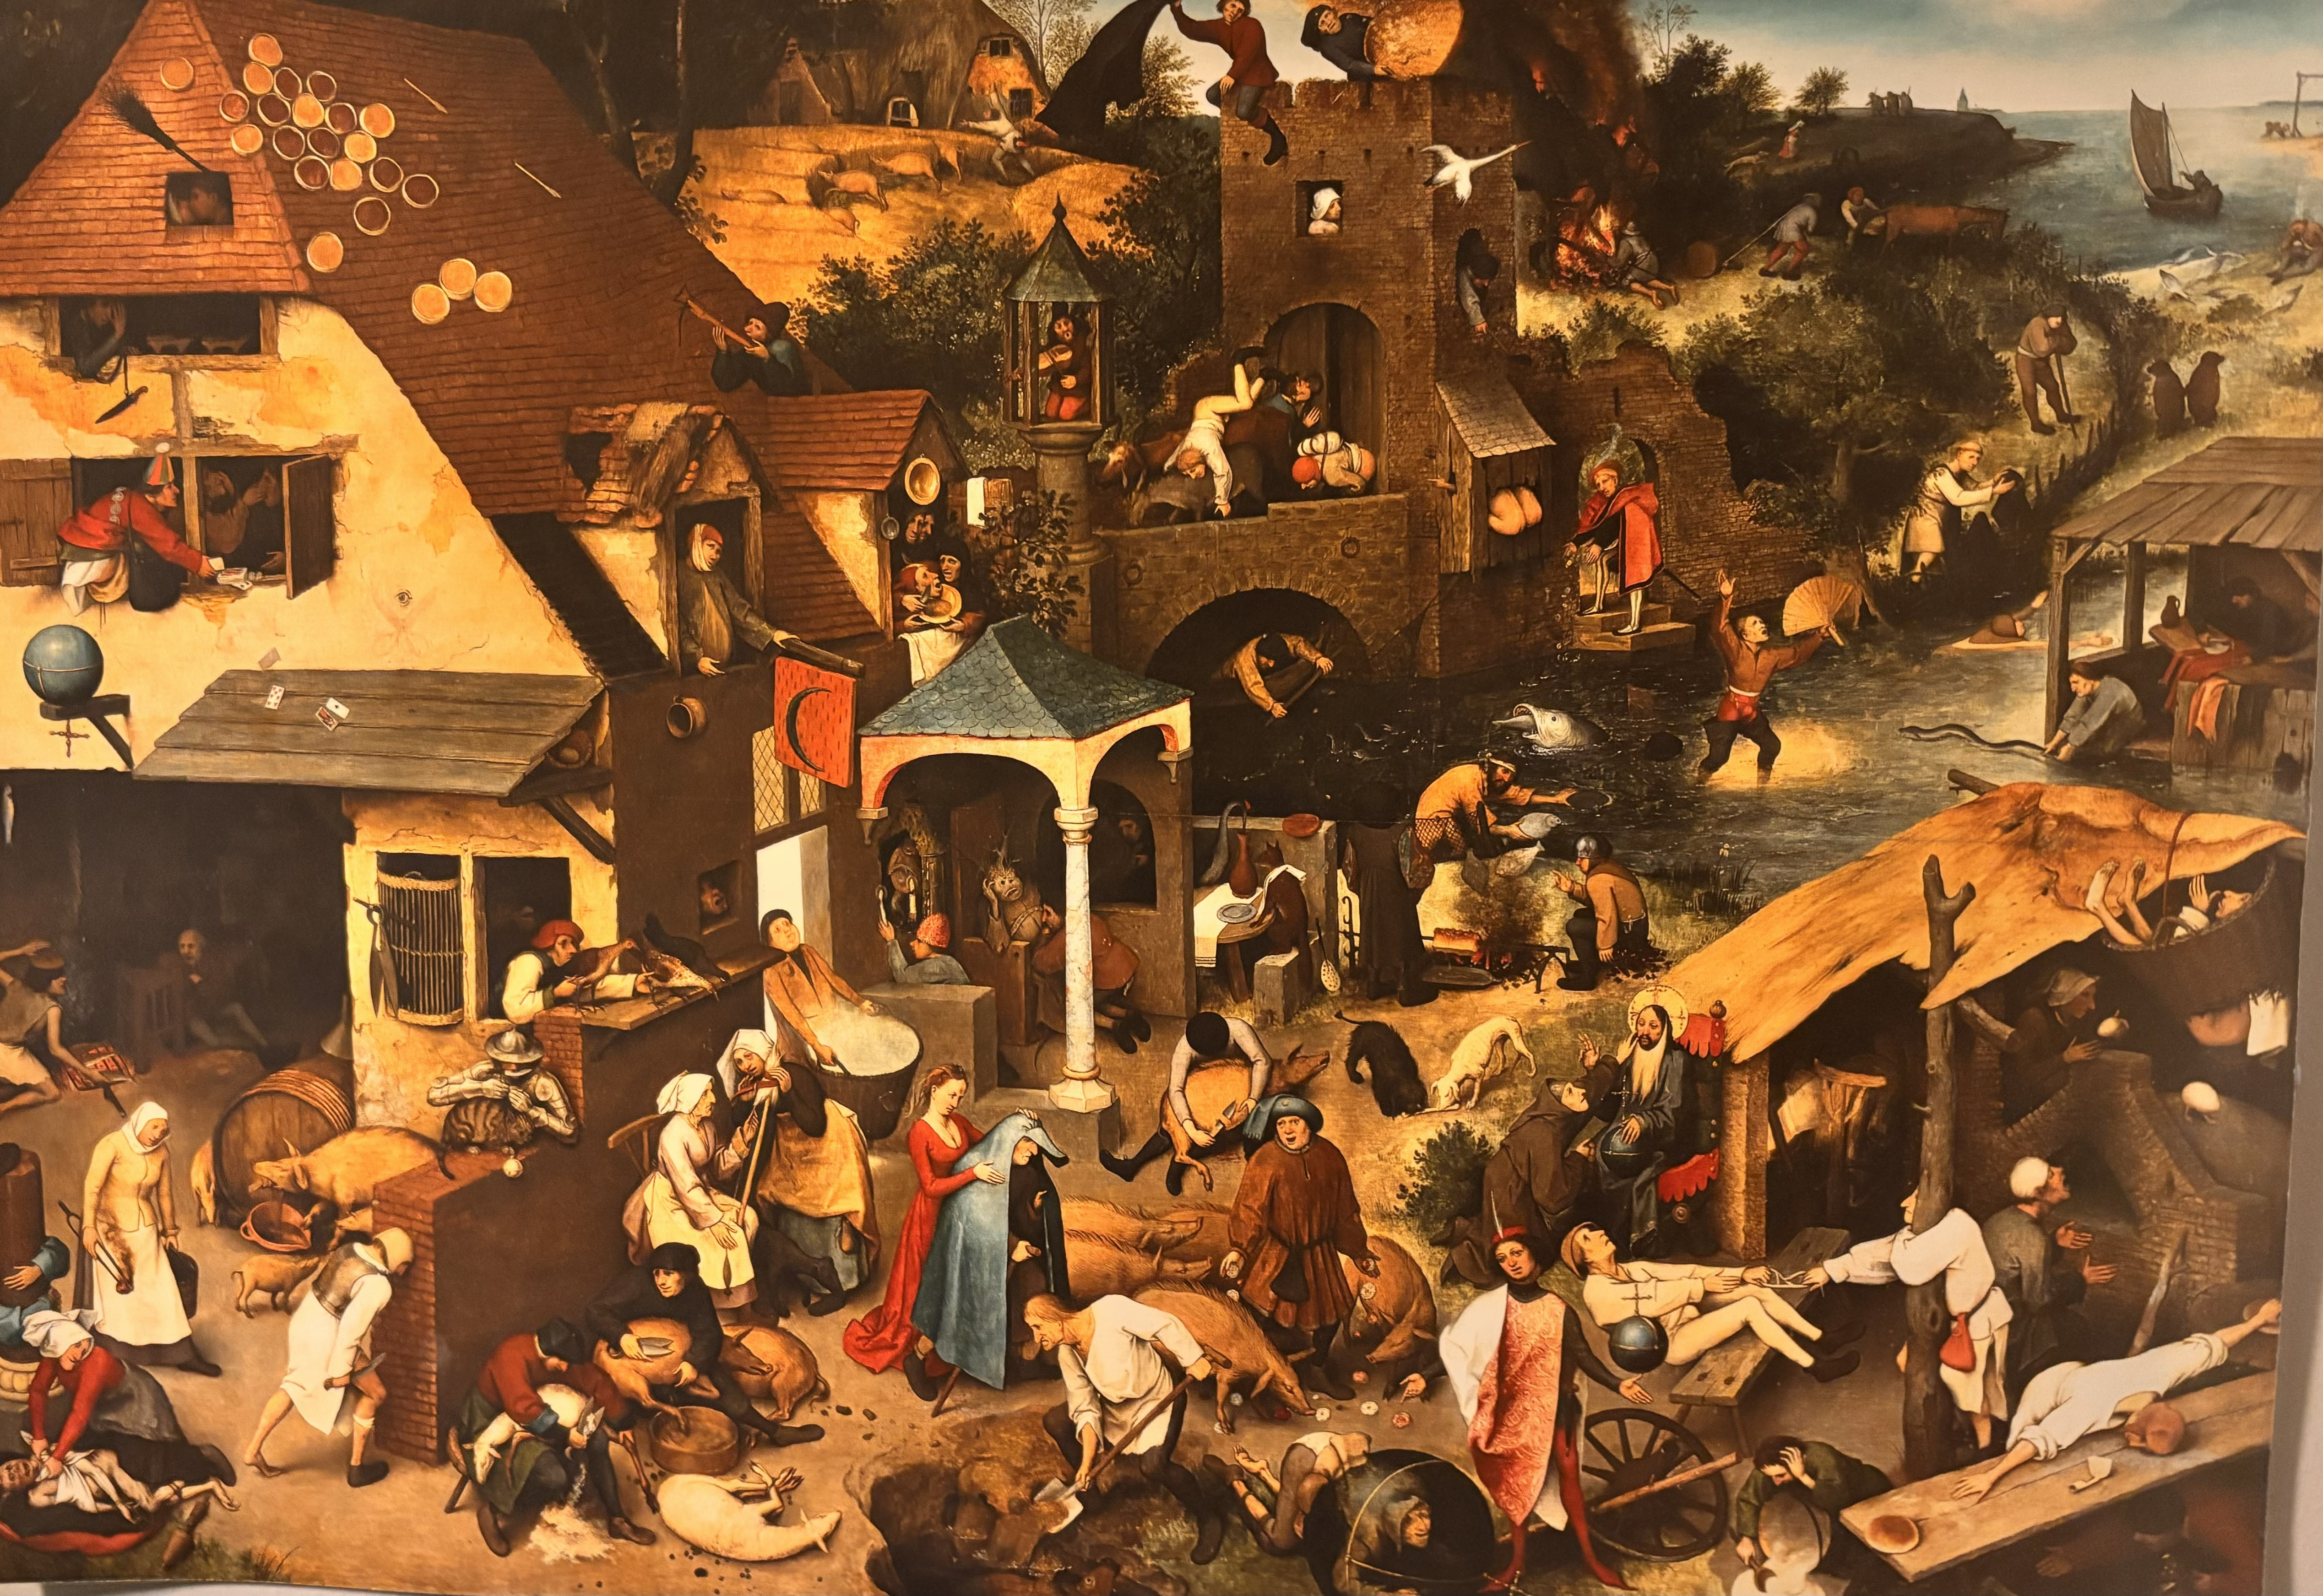
\includegraphics[width = \textwidth]{chapter8/IMG_ch8/proverbe} \caption{Pieter Bruegel’s Netherlandish Proverbs (oil on wood, painted 1559). For years, this painting has fascinated me. One of the reasons is that it was painted in a time still marred by plagues. Enough time had persisted since the first wave in 1345 for the societal upheaval to become fully manifest. Above all, it appears to depict a time in which the previous structures, customs, and societal norms are in complete disarray. A time of flux and dynamism, perhaps representative of what Nietzsche said in the quote referenced above: \ \noindent"At this turning-point of history there manifest themselves, side by side, and often mixed and entangled together, a magnificent, manifold, virgin-forest-like up-growth and up-striving, a kind of tropical tempo in the rivalry of growth, and an extraordinary decay and self-destruction, owing to the savagely opposing and seemingly exploding egoisms, which strive with one another 'for sun and light.'"} \label{redone} \end{figure}





\begin{figure}[H] 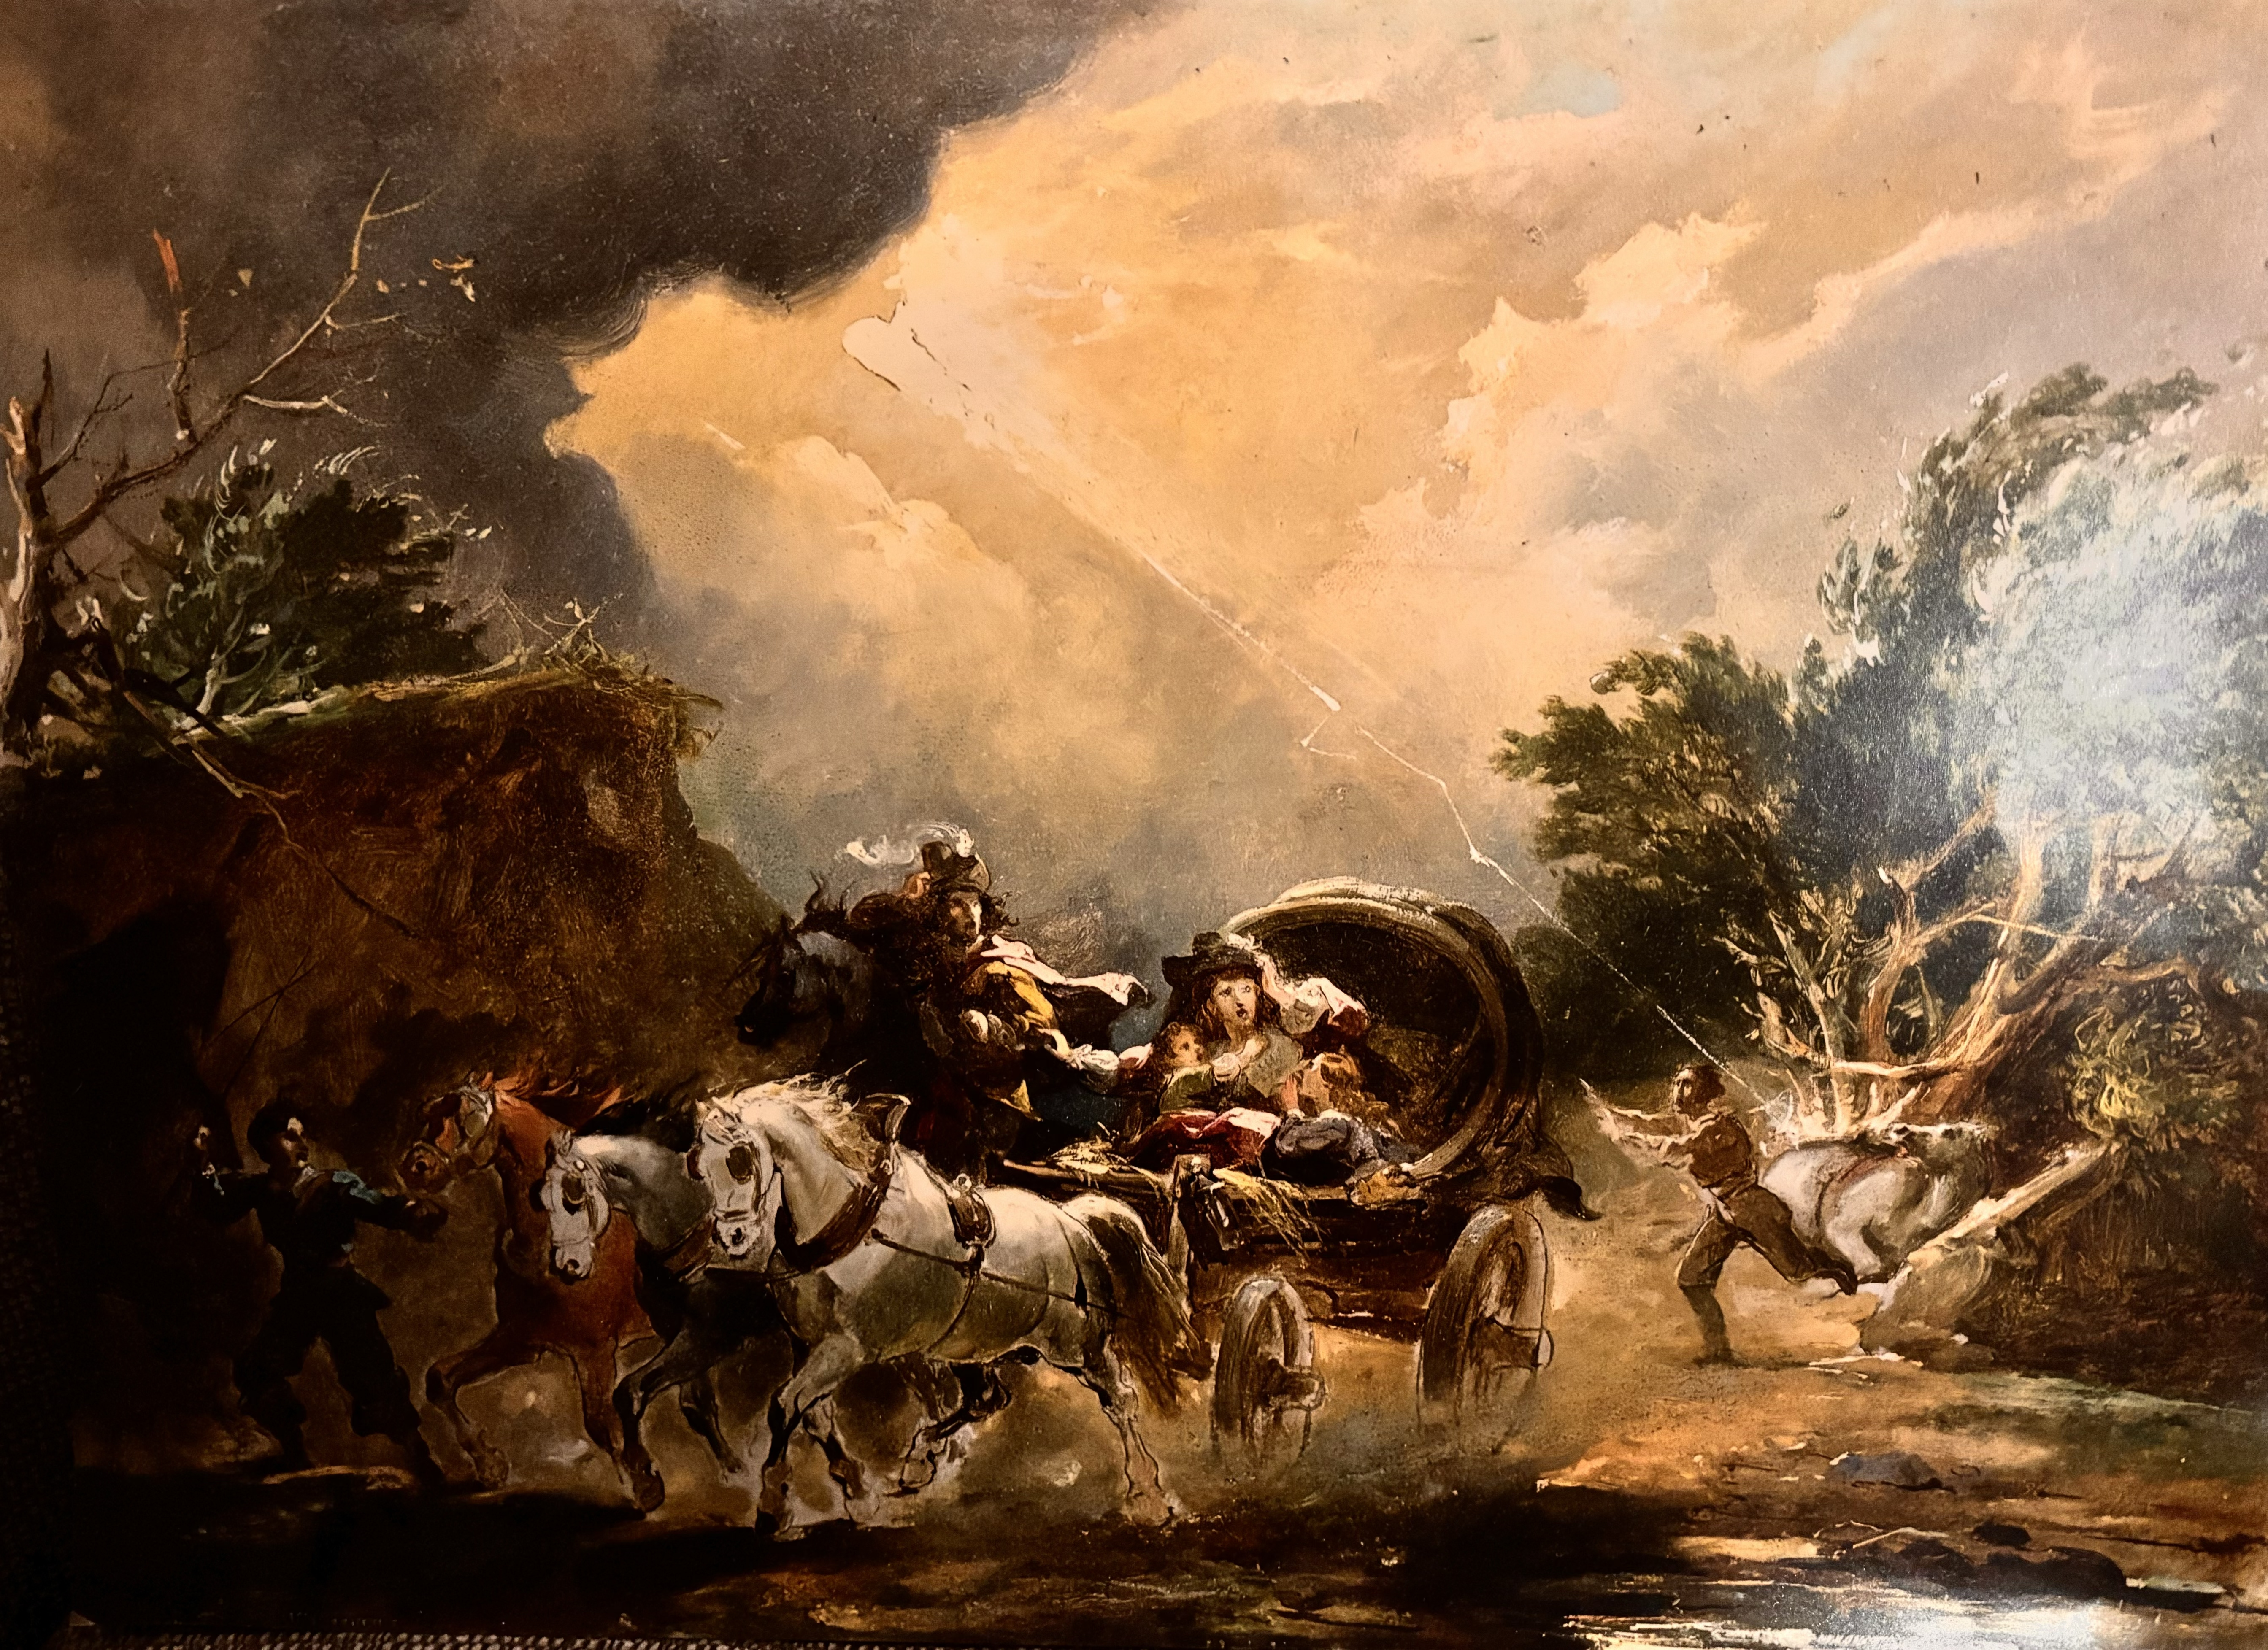
\includegraphics[width = \textwidth]{lightning}
\centering
\pagebreak \caption{Coach in a Thunderstorm (Philippe Jacques de Loutherbourg, 1790).  It almost appears as if the cart, the horse and the person are eminating from the lightning strike,  rather than merely running away from it after being struck on the road. As if the energy of the lightning itself is creating the activity we see before us.  We have no way of knowing whether Philippe Jacques intended for this this interpretation.  But the emergences of sudden complex order through immediate resolutions of large potential,  seems like it might be consistent with the situaten of  a country (France) at the verge of instability,  which ultimately manifested into full blown societal revolution only a few years later.  To be clear, I am suggesting the interpretation that the motion depected is an ephemeral dissipative structure,  momentarily created by the lightning. } \label{redone} \end{figure}








\section{Birth-plague model}

Birth
$$\pr{\Delta \xt = 1, \Delta \yt = 0} = \beta \xt \Delta t +o(\Delta t)$$
Corruption (instantiation of plague)
$$\pr{\Delta \xt = -1, \Delta \yt = 1} = \delta \xt \Delta t +o(\Delta t)$$
Infection (spreading of plague)
$$\pr{\Delta \xt = -1, \Delta \yt = 1} = \alpha \xt\yt \Delta t +o(\Delta t)$$
Dying (death of plague infected)
$$\pr{\Delta \xt = 0, \Delta \yt = -1} = \mu \yt \Delta t +o(\Delta t)$$
No event
$$\pr{\Delta \xt = \Delta \yt = 0} =1 - \lrbs{(\beta + \delta + \alpha \yt) \xt + \mu \yt} \Delta t +o(\Delta t)$$





\begin{figure}[h!]
    \centering
    % First row
    \begin{subfigure}{0.49\textwidth}
        \centering
        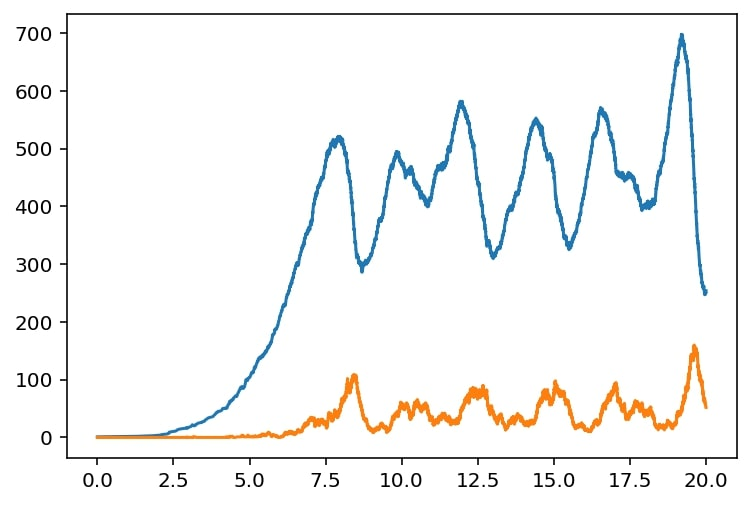
\includegraphics[width=\linewidth]{bpPLOT}
        \label{fig:figure1}
    \end{subfigure}
    \hfill
    \begin{subfigure}{0.49\textwidth}
        \centering
        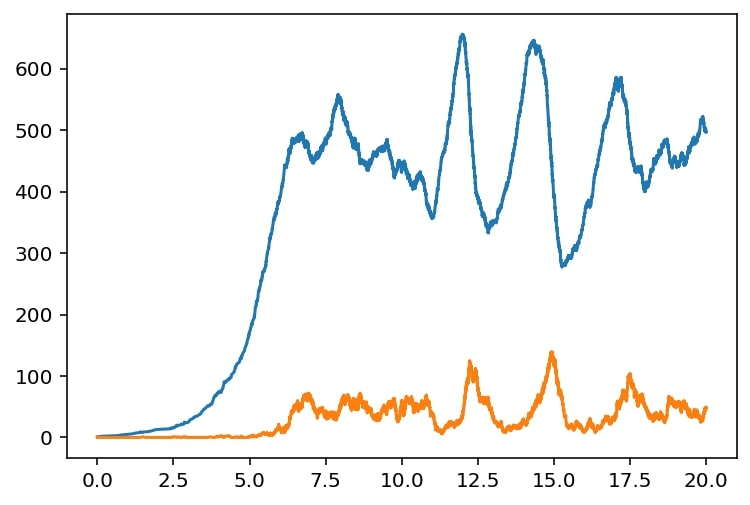
\includegraphics[width=\linewidth]{bpPLOT2}
        \label{fig:figure2}
    \end{subfigure}
    
    % Second row
    \vspace{0.5cm} % Optional: adds some space between rows
    \begin{subfigure}{0.49\textwidth}
        \centering
        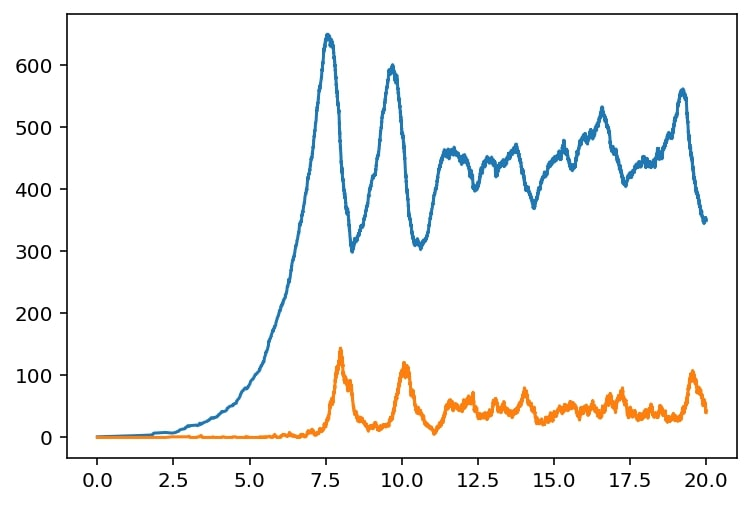
\includegraphics[width=\linewidth]{bpPLOT3}
        \label{fig:figure3}
    \end{subfigure}
    \hfill
    \begin{subfigure}{0.49\textwidth}
        \centering
        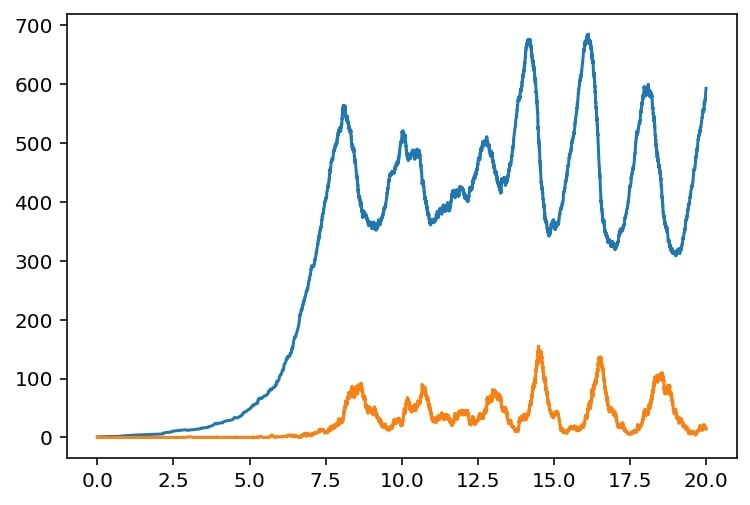
\includegraphics[width=\linewidth]{bpPLOT4}
        \label{fig:figure4}
    \end{subfigure}
    
    \caption{($\beta, \delta, \alpha, \mu$) = (birth, corruption, infection , dying) = (1, 0.1, 0.02, 10). Four realisations of the birth plague model. In each, the blue line is $\xt$ (population count), $\yt$ is the number of plague infected individuals.}
    \label{fig:four-figures}
\end{figure}




\section{(Density dependent) Vitallity birth-plague model}

To attempt to illustrate the cyclic phases of multiplicative bifurcation, waining, colapse, and re-sustaining development as seen in both turbulence shedding, and the rise and often suddern fall of living dissipative structures at multiple scales. \par 

\vspace{10pt}
This model is a combination of the previous two (birth-plague and RRRR).  It incorporates the idea from RRRR that catastrophe (but in this case plague instantiation) is driven by a situation of relative per capita scarcity (per capita reffering to the multiplicative agencies brought about by successive bifurcations).  This, general concept, in principle being at least artistically applicative to multiple phenomena,  but notably, the dissipative structures of fluid turbulence shedding and population collapse. 

This model is a combination of the previous two (birth-plague and RRRR). It incorporates the idea from RRRR that catastrophe (in this case, plague instantiation) is driven by a situation of relative per capita scarcity (per capita referring to the multiplicative agencies brought about by successive bifurcations). This general concept is, in principle, at least artistically applicable to multiple phenomena, but notably to the dissipative structures of fluid turbulence shedding and population collapse.

(Potential availability)
 $$\ddt{V} = \xi - p \xt$$
Birth
$$\pr{\Delta \xt = 1, \Delta \yt = 0} = \beta \xt \Delta t +o(\Delta t)$$
Corruption (instantiation of plague)
$$\pr{\Delta \xt = -1, \Delta \yt = 1} = \delta \xt \Delta t +o(\Delta t)$$
Infection (spreading of plague)
$$\pr{\Delta \xt = -1, \Delta \yt = 1} = \alpha \xt\yt \Delta t +o(\Delta t)$$
Dying (death of plague infected)
$$\pr{\Delta \xt = 0, \Delta \yt = -1} = \mu \yt \Delta t +o(\Delta t)$$
No event
$$\pr{\Delta \xt = \Delta \yt = 0} =1 - \lrbs{(\beta + \delta + \alpha \yt) \xt + \mu \yt} \Delta t +o(\Delta t)$$





\subsection*{Plague in popular culture}

\textbf{Roses poem:}\\

\begin{center}
"Ring-a-ring o’ roses\\
A pocket full of posies;\\
Atishoo, atishoo,\\
We all fall down."
\end{center}

\noindent
\textbf{Edgar Allen Poe -- The masque of the red death}
\begin{center}
\begin{quotation}
\noindent
``All these and security were within. Without was the “Red Death.” \cite{poe2020masque}\\

\noindent
\hfill \dots \hfill\\

\noindent
It was toward the close of the fifth or sixth month of his seclusion, and while the pestilence raged
most furiously abroad, that the Prince Prospero entertained his thousand friends at a masked ball of the
most unusual magnificence.
It was a voluptuous scene, that masquerade.\\

\noindent
\hfill \dots \hfill  \\

\noindent
And thus too, it happened, perhaps, that before
the last echoes of the last chime had utterly sunk into silence, there were many individuals in the crowd
who had found leisure to become aware of the presence of a masked figure which had arrested the
attention of no single individual before. And the rumor of this new presence having spread itself
whisperingly around, there arose at length from the whole company a buzz, or murmur, expressive of
disapprobation and surprise — then, finally, of terror, of horror, and of disgust.\\

\noindent
\hfill \dots \hfill \\

\noindent
And now was acknowledged the presence of the Red Death. He had come like a thief in the night.
And one by one dropped the revellers in the blood-bedewed halls of their revel, and died each in the
despairing posture of his fall. And the life of the ebony clock went out with that of the last of the gay.
And the flames of the tripods expired. And Darkness and Decay and the Red Death held illimitable
dominion over all."
\end{quotation}
\end{center}


%%%%%%%%%%%%%%%%%%%%%%%%%%%%%%%%%%%%%%%%%%%%%%%%%%%%%%%%%%%%555


















































